\documentclass[12pt,letterpaper]{article}

% =========================
% Paquetes
% =========================
\usepackage[utf8]{inputenc}
\usepackage[T1]{fontenc}
\usepackage[spanish,es-tabla]{babel}
\usepackage{geometry}
\usepackage{setspace}
\usepackage{graphicx}
\usepackage{xcolor}
\usepackage{array}
\usepackage{longtable}
\usepackage{booktabs}
\usepackage{tabularx}
\usepackage{float}
\usepackage{hyperref}
\usepackage{fancyhdr}
\usepackage{caption}
\usepackage{enumitem}
\usepackage{multirow}
\usepackage{lastpage}
\usepackage{tocloft}

% =========================
% Configuración general
% =========================
\geometry{left=2.8cm,right=2.8cm,top=2.6cm,bottom=2.6cm}
\onehalfspacing
\setlength{\parskip}{0.5em}
\setlength{\parindent}{0pt}
\setlength{\cftsecnumwidth}{2.8em}
\sloppy
\emergencystretch=2em

\hypersetup{
    colorlinks=true,
    linkcolor=black,
    urlcolor=blue,
    citecolor=black
}

\pagestyle{fancy}
\fancyhf{}
\setlength{\headheight}{14.5pt}
\lhead{AUT/UAT: Secure Ticket}
\rhead{\thepage}
\renewcommand{\headrulewidth}{0.4pt}
\renewcommand{\tablename}{Tabla}

\captionsetup{font=small,labelfont=bf}

% =========================
% Comandos editables
% =========================
\newcolumntype{L}[1]{>{\raggedright\arraybackslash}p{#1}}
\newcolumntype{C}[1]{>{\centering\arraybackslash}p{#1}}
\newcolumntype{Y}{>{\raggedright\arraybackslash}X}

\newcommand{\CampoEditable}[1]{\textcolor{blue}{#1}}

\newcommand{\NombreProyecto}{Secure Ticket}
\newcommand{\NombreDocumento}{Documento de Pruebas de Aceptación de Usuario}
\newcommand{\SubtituloProyecto}{Pruebas AUT/UAT para la validación funcional del prototipo}
\newcommand{\VersionDocumento}{1.3 final}
\newcommand{\FechaDocumento}{22 de mayo de 2026}

\newcommand{\Institucion}{Pontificia Universidad Javeriana}
\newcommand{\Facultad}{Facultad de Ingeniería}
\newcommand{\Programa}{Ingeniería de Sistemas}
\newcommand{\Ciudad}{Bogotá, D.C.}

% =========================
% Documento
% =========================
\begin{document}

% =========================
% Portada
% =========================
\hypersetup{pageanchor=false}
\begin{titlepage}
    \thispagestyle{empty}
    \centering
    \begingroup
    \setlength{\parskip}{0pt}

    \vspace*{-0.2cm}

    {\Large \textbf{\NombreDocumento}\par}
    \vspace{0.45cm}

    {\Large \NombreProyecto\par}
    \vspace{0.35cm}

    {\normalsize \SubtituloProyecto\par}
    \vspace{0.85cm}

    {\normalsize Versión \VersionDocumento{} --- \FechaDocumento\par}

    \vspace{0.9cm}

    \IfFileExists{Logo Javeriana.png}{
        
\includegraphics[width=3.4cm]{Logo Javeriana.png}
    }{
        \fbox{\parbox[c][3.4cm][c]{3.4cm}{\centering Logo}}
    }

    \vspace{1.1cm}

    {\normalsize Juan Diego Arias Durán\par}
    \vspace{0.18cm}
    {\normalsize Santiago Andrés Mesa Niño\par}
    \vspace{0.18cm}
    {\normalsize Andrés Felipe Manosalva Garzón\par}
    \vspace{0.18cm}
    {\normalsize Juan Camilo Carvajal Rodríguez\par}

    \vspace{1.0cm}

    {\normalsize Presentado al director\par}
    \vspace{0.25cm}
    {\normalsize Rafael Vicente Páez Méndez, PhD\par}

    \vfill

    {\normalsize \Institucion\par}
    \vspace{0.12cm}
    {\normalsize \Facultad\par}
    \vspace{0.12cm}
    {\normalsize \Programa\par}
    \vspace{0.12cm}
    {\normalsize \Ciudad\par}
    \vspace{0.12cm}
    {\normalsize \the\year\par}

    \endgroup
\end{titlepage}
\hypersetup{pageanchor=true}

% =========================
% Historial de cambios
% =========================

\section*{Historial de cambios}
\addcontentsline{toc}{section}{Historial de cambios}

\begin{table}[H]
\centering
\begingroup
\footnotesize
\setlength{\tabcolsep}{3pt}
\renewcommand{\arraystretch}{1.25}

\begin{tabularx}{\textwidth}{|
>{\centering\arraybackslash}p{1.8cm}|
>{\centering\arraybackslash}p{2.5cm}|
>{\raggedright\arraybackslash}p{4.0cm}|
>{\raggedright\arraybackslash}X|}
\hline
\multicolumn{1}{|>{\centering\arraybackslash}m{1.8cm}|}{\textbf{Versión}} &
\multicolumn{1}{>{\centering\arraybackslash}m{2.5cm}|}{\textbf{Fecha}} &
\multicolumn{1}{>{\centering\arraybackslash}m{4.0cm}|}{\textbf{Sección modificada}} &
\multicolumn{1}{>{\centering\arraybackslash}m{6.3cm}|}{\textbf{Descripción de cambios}} \\
\hline
1.0 &
21/05/2026 &
Documento completo &
Versión inicial del documento de pruebas de aceptación de usuario AUT/UAT para Secure Ticket. \\
\hline
1.1 &
22/05/2026 &
Resultados AUT/UAT &
Diligenciamiento de casos de prueba, participantes, registro de ejecución, resultados, trazabilidad, decisión de aceptación y anexos. \\
\hline
1.2 final &
22/05/2026 &
Versión final &
Actualización del ambiente desplegado, consolidado final de respuestas, explicación de valores no aplicables, ajuste de anexos y eliminación de referencias a formularios individuales o actas formales. \\
\hline
1.3 final &
22/05/2026 &
Revisión final AUT/UAT &
Ajuste de redacción académica, precisión metodológica en escenarios de reventa, aclaración del cálculo del promedio de satisfacción, corrección del índice y fortalecimiento de la sección de anexos. \\
\hline
\end{tabularx}

\endgroup
\caption{Historial de cambios del documento AUT/UAT}
\label{tab:historial-cambios-uat}
\end{table}
\newpage

% =========================
% Índices
% =========================
\tableofcontents
\newpage

\listoftables
\newpage

% =========================
% 1. Introducción
% =========================
\section{Introducción}

\subsection{Propósito del documento}

El propósito de este documento es definir, organizar y registrar las pruebas de aceptación de usuario del sistema \NombreProyecto{}. Estas pruebas permiten validar, desde la perspectiva de usuarios o interesados representativos, que el prototipo satisface los flujos funcionales principales definidos para el trabajo de grado.

El documento establece el alcance de la aceptación, los perfiles participantes, los escenarios evaluados, los criterios de entrada y salida, los casos de prueba, los instrumentos de recolección de información, los resultados obtenidos y la decisión final de aceptación del sistema.

\subsection{Alcance del documento}

Este documento cubre las pruebas de aceptación asociadas a los flujos principales de \NombreProyecto{}, incluyendo:

\begin{itemize}[leftmargin=*]
    \item Inicio de sesión y acceso al sistema según rol.
    \item Consulta de eventos disponibles.
    \item Compra primaria simulada de tickets.
    \item Consulta del inventario de tickets del usuario.
    \item Publicación de tickets para reventa.
    \item Compra de tickets en reventa.
    \item Verificación de tickets mediante código QR.
    \item Validación de restricciones por rol, propiedad y estado del ticket.
\end{itemize}

Las pruebas se realizan en un ambiente académico controlado. No se incluye operación en producción, uso de dinero real, despliegue en Stellar Mainnet, integración con pasarelas de pago reales ni procesos KYC/AML.

\subsection{Audiencia objetivo}

Este documento está dirigido a:

\begin{itemize}[leftmargin=*]
    \item Equipo de desarrollo frontend, backend y contratos inteligentes.
    \item Equipo responsable de pruebas, validación y documentación.
    \item Director del trabajo de grado.
    \item Jurados o revisores académicos.
    \item Usuarios o interesados participantes en la validación.
\end{itemize}

\subsection{Referencias}

\begin{table}[H]
\centering
\begingroup
\footnotesize
\setlength{\tabcolsep}{3pt}
\renewcommand{\arraystretch}{1.25}

\begin{tabularx}{\textwidth}{|
>{\centering\arraybackslash}p{1.5cm}|
>{\raggedright\arraybackslash}X|}
\hline
\multicolumn{1}{|>{\centering\arraybackslash}m{1.5cm}|}{\textbf{ID}} &
\multicolumn{1}{>{\centering\arraybackslash}m{12.7cm}|}{\textbf{Referencia}} \\
\hline
R1 & Especificación de Requerimientos de Software de Secure Ticket. \\
\hline
R2 & Documento de Arquitectura o Diseño de Software de Secure Ticket. \\
\hline
R3 & Plan de Pruebas de Secure Ticket. \\
\hline
R4 & ISO/IEC/IEEE 29148:2018, Systems and software engineering -- Life cycle processes -- Requirements engineering. \\
\hline
R5 & Evidencias funcionales, técnicas y de ejecución del prototipo Secure Ticket. \\
\hline
\end{tabularx}

\endgroup
\caption{Referencias utilizadas en el documento AUT/UAT}
\label{tab:referencias-uat}
\end{table}

% =========================
% 2. Definiciones
% =========================
\section{Definiciones, acrónimos y abreviaciones}

\begin{table}[H]
\centering
\begingroup
\footnotesize
\setlength{\tabcolsep}{3pt}
\renewcommand{\arraystretch}{1.25}

\begin{tabularx}{\textwidth}{|
>{\raggedright\arraybackslash}p{3.4cm}|
>{\raggedright\arraybackslash}X|}
\hline
\multicolumn{1}{|>{\centering\arraybackslash}m{3.4cm}|}{\textbf{Término}} &
\multicolumn{1}{>{\centering\arraybackslash}m{10.8cm}|}{\textbf{Definición}} \\
\hline
AUT & Pruebas de aceptación de usuario. En este documento se usa como denominación complementaria a UAT para referirse a la validación ejecutada por usuarios o interesados representativos. \\
\hline
UAT & User Acceptance Testing. Pruebas orientadas a validar si el sistema satisface las necesidades funcionales y operativas esperadas por los usuarios finales o interesados. \\
\hline
Stakeholder & Persona, grupo u organización con interés en el sistema, sus resultados o su operación. \\
\hline
Escenario de aceptación & Flujo funcional representativo que será ejecutado durante la prueba para validar el comportamiento del sistema. \\
\hline
Criterio de aceptación & Condición observable que debe cumplirse para considerar aceptado un flujo, requerimiento o funcionalidad. \\
\hline
Defecto & Comportamiento incorrecto, incompleto o inesperado identificado durante la ejecución de la prueba. \\
\hline
Incidencia bloqueante & Defecto que impide completar un flujo crítico de aceptación. \\
\hline
Ticket & Entrada digital asociada a un evento, gestionada por el sistema y vinculada a un estado dentro del ciclo de vida de la boleta. \\
\hline
Reventa & Proceso mediante el cual un usuario publica un ticket adquirido para que otro usuario pueda comprarlo en el mercado secundario del prototipo. \\
\hline
Escáner QR & Módulo que permite validar el estado de un ticket mediante la lectura o ingreso de un código QR. \\
\hline
\end{tabularx}

\endgroup
\caption{Definiciones, acrónimos y abreviaciones}
\label{tab:definiciones-uat}
\end{table}

% =========================
% 3. Objetivos
% =========================
\section{Objetivos de las pruebas de aceptación}

\subsection{Objetivo general}

Validar que el prototipo \NombreProyecto{} cumple con los flujos funcionales principales esperados por usuarios e interesados, de acuerdo con el alcance académico del proyecto y los requerimientos definidos para la solución.

\subsection{Objetivos específicos}

\begin{itemize}[leftmargin=*]
    \item Verificar que los usuarios puedan completar los flujos principales del sistema sin errores bloqueantes.
    \item Evaluar la comprensión de la interfaz y de los mensajes presentados por el sistema.
    \item Validar que el sistema comunica adecuadamente el estado de los tickets.
    \item Comprobar que los flujos de compra, reventa y verificación resultan comprensibles para los participantes.
    \item Identificar defectos funcionales, problemas de usabilidad o brechas de aceptación antes de la entrega final.
    \item Obtener evidencia formal de aceptación o aceptación condicionada del prototipo.
\end{itemize}

% =========================
% 4. Alcance
% =========================
\section{Alcance de las pruebas AUT/UAT}

\subsection{Funcionalidades incluidas}

\begin{table}[H]
\centering
\begingroup
\footnotesize
\setlength{\tabcolsep}{3pt}
\renewcommand{\arraystretch}{1.25}

\begin{tabularx}{\textwidth}{|
>{\centering\arraybackslash}p{2.2cm}|
>{\raggedright\arraybackslash}X|
>{\centering\arraybackslash}p{2.8cm}|}
\hline
\multicolumn{1}{|>{\centering\arraybackslash}m{2.2cm}|}{\textbf{ID}} &
\multicolumn{1}{>{\centering\arraybackslash}m{8.8cm}|}{\textbf{Funcionalidad}} &
\multicolumn{1}{>{\centering\arraybackslash}m{2.8cm}|}{\textbf{Estado en UAT}} \\
\hline
UAT-F01 & Inicio de sesión y acceso al sistema según rol. & Incluida \\
\hline
UAT-F02 & Consulta de eventos disponibles. & Incluida \\
\hline
UAT-F03 & Compra primaria simulada de ticket. & Incluida \\
\hline
UAT-F04 & Consulta del inventario de tickets del usuario. & Incluida \\
\hline
UAT-F05 & Publicación de ticket para reventa. & Incluida \\
\hline
UAT-F06 & Compra de ticket en reventa. & Incluida \\
\hline
UAT-F07 & Verificación de ticket mediante código QR. & Incluida \\
\hline
UAT-F08 & Restricciones por rol, propiedad y estado del ticket. & Incluida \\
\hline
\end{tabularx}

\endgroup
\caption{Funcionalidades incluidas en las pruebas AUT/UAT}
\label{tab:funcionalidades-uat}
\end{table}

\subsection{Elementos fuera del alcance}

Quedan fuera del alcance de estas pruebas:

\begin{itemize}[leftmargin=*]
    \item Pagos reales con dinero fiat.
    \item Integración productiva con pasarelas de pago.
    \item Operación en Stellar Mainnet.
    \item Pruebas legales o comerciales sobre operación real de boletería.
    \item Validación de usuarios mediante procesos KYC/AML.
    \item Pruebas masivas con usuarios reales en eventos físicos.
    \item Pruebas de rendimiento sobre transacciones blockchain reales en condiciones productivas.
\end{itemize}

\subsection{Suposiciones y restricciones}

\begin{itemize}[leftmargin=*]
    \item Los participantes ejecutan las pruebas en un ambiente controlado.
    \item El sistema se encuentra disponible en el ambiente de staging definido para AUT/UAT, compuesto por frontend en Vercel, backend en Railway, base de datos PostgreSQL/Supabase y Stellar/Soroban Testnet para los escenarios que involucren interacción blockchain.
    \item Las cuentas, eventos y tickets de prueba son creados previamente por el equipo.
    \item Los usuarios no necesitan conocimientos técnicos sobre blockchain para ejecutar los escenarios.
    \item La evaluación se enfoca en aceptación funcional y usabilidad básica, no en certificación productiva.
    \item Las pruebas blockchain se limitan al alcance implementado en el prototipo y al uso de Stellar/Soroban Testnet en los escenarios que involucren contratos, transacciones firmadas, eventos on-chain o hashes de transacción.
    \end{itemize}

% =========================
% 5. Participantes
% =========================
\section{Participantes y roles}

\subsection{Perfiles participantes}

\begin{table}[H]
\centering
\begingroup
\footnotesize
\setlength{\tabcolsep}{3pt}
\renewcommand{\arraystretch}{1.25}

\begin{tabularx}{\textwidth}{|
>{\raggedright\arraybackslash}p{2.8cm}|
>{\raggedright\arraybackslash}p{4.2cm}|
>{\raggedright\arraybackslash}X|}
\hline
\multicolumn{1}{|>{\centering\arraybackslash}m{2.8cm}|}{\textbf{Perfil}} &
\multicolumn{1}{>{\centering\arraybackslash}m{4.2cm}|}{\textbf{Descripción}} &
\multicolumn{1}{>{\centering\arraybackslash}m{7.0cm}|}{\textbf{Actividades esperadas}} \\
\hline
Comprador & Usuario que adquiere tickets para eventos. & Comprar ticket, consultar inventario y revisar estado del ticket. \\
\hline
Vendedor & Usuario que publica un ticket para reventa. & Listar ticket en reventa y validar cambio de estado. \\
\hline
Staff & Usuario encargado de verificar tickets. & Escanear código QR y validar estado del ticket. \\
\hline
Administrador & Usuario con permisos de gestión. & Revisar información de eventos, tickets o usuarios según el alcance implementado. \\
\hline
Stakeholder académico & Evaluador o interesado del proyecto. & Observar el flujo, emitir retroalimentación y validar cumplimiento general. \\
\hline
\end{tabularx}

\endgroup
\caption{Perfiles participantes en AUT/UAT}
\label{tab:perfiles-participantes-uat}
\end{table}

\subsection{Responsabilidades}

\begin{table}[H]
\centering
\begingroup
\footnotesize
\setlength{\tabcolsep}{3pt}
\renewcommand{\arraystretch}{1.25}

\begin{tabularx}{\textwidth}{|
>{\raggedright\arraybackslash}p{3.5cm}|
>{\raggedright\arraybackslash}X|}
\hline
\multicolumn{1}{|>{\centering\arraybackslash}m{3.5cm}|}{\textbf{Rol}} &
\multicolumn{1}{>{\centering\arraybackslash}m{10.7cm}|}{\textbf{Responsabilidad}} \\
\hline
Equipo de pruebas & Preparar ambiente, datos, guion de prueba, formularios y registro de resultados. \\
\hline
Participante UAT & Ejecutar los escenarios asignados y responder el instrumento de aceptación. \\
\hline
Observador & Registrar incidencias, tiempos, bloqueos y comentarios relevantes. \\
\hline
Equipo de desarrollo & Analizar defectos identificados y definir acciones correctivas si aplica. \\
\hline
Director/Revisor & Evaluar la pertinencia de los resultados como evidencia académica. \\
\hline
\end{tabularx}

\endgroup
\caption{Responsabilidades durante la ejecución AUT/UAT}
\label{tab:responsabilidades-uat}
\end{table}

% =========================
% 6. Ambiente
% =========================
\section{Ambiente de prueba}

\subsection{Configuración del ambiente}

\begin{table}[H]
\centering
\begingroup
\footnotesize
\setlength{\tabcolsep}{3pt}
\renewcommand{\arraystretch}{1.25}

\begin{tabularx}{\textwidth}{|
>{\raggedright\arraybackslash}p{3.5cm}|
>{\raggedright\arraybackslash}X|}
\hline
\multicolumn{1}{|>{\centering\arraybackslash}m{3.5cm}|}{\textbf{Elemento}} &
\multicolumn{1}{>{\centering\arraybackslash}m{10.7cm}|}{\textbf{Descripción}} \\
\hline
Frontend & Aplicación web desplegada en Vercel: \texttt{https://stellar-ticket-staging.vercel.app}. Este ambiente se usa para la validación manual de los flujos visibles por usuarios finales. \\
\hline
Backend/API & API desplegada en Railway: \texttt{https://stellar-tickets-staging.up.railway.app}. Las rutas principales se exponen bajo \texttt{/api}; el endpoint de salud es \texttt{/health}. \\
\hline
Base de datos & PostgreSQL/Supabase en ambiente de pruebas o staging, usando el schema \texttt{ticketing}. Almacena usuarios, eventos, órdenes, tickets, check-ins, reclamos PQR y proyecciones operativas del indexador. \\
\hline
Blockchain & Stellar/Soroban Testnet para validaciones manuales que involucren contratos, transacciones firmadas, eventos on-chain y hashes de transacción. \\
\hline
Wallet & Freighter Wallet configurada en Testnet. Se usa para pruebas manuales de conexión de wallet, firma y envío de transacciones cuando el escenario lo requiere. \\
\hline
Navegador & Google Chrome con Freighter instalado para pruebas manuales. Para validaciones automatizadas de interfaz se usa Chromium mediante Playwright cuando aplica. \\
\hline
Dispositivo & Computador portátil con acceso a internet para ejecutar la sesión UAT sobre los ambientes desplegados. \\
\hline
Sistema operativo & macOS. \\
\hline
\end{tabularx}

\endgroup
\caption{Configuración del ambiente AUT/UAT}
\label{tab:configuracion-ambiente-uat}
\end{table}

\subsection{Datos de prueba}

\begin{table}[H]
\centering
\begingroup
\footnotesize
\setlength{\tabcolsep}{3pt}
\renewcommand{\arraystretch}{1.25}

\begin{tabularx}{\textwidth}{|
>{\raggedright\arraybackslash}p{3.3cm}|
>{\raggedright\arraybackslash}p{4.4cm}|
>{\raggedright\arraybackslash}X|}
\hline
\multicolumn{1}{|>{\centering\arraybackslash}m{3.3cm}|}{\textbf{Dato}} &
\multicolumn{1}{>{\centering\arraybackslash}m{4.4cm}|}{\textbf{Valor o ejemplo}} &
\multicolumn{1}{>{\centering\arraybackslash}m{6.5cm}|}{\textbf{Uso}} \\
\hline
Usuario comprador & \texttt{comprador@test.com} & Compra primaria simulada, consulta de órdenes, visualización de tickets y validación de acceso como cliente. \\
\hline
Usuario vendedor & \texttt{vendedor@test.com} & Publicación o validación de tickets en escenarios de reventa, cuando el flujo esté habilitado para el evento probado. \\
\hline
Usuario staff & \texttt{staff@test.com} & Verificación de tickets mediante QR desde el módulo de escáner operativo. \\
\hline
Usuario administrador & \texttt{admin@test.com} & Gestión y revisión de información administrativa según permisos: eventos, políticas, contratos, reclamos y operación general. \\
\hline
Evento de prueba & Evento disponible en el ambiente desplegado de Vercel/Railway. & Flujo de compra primaria simulada, consulta de catálogo, emisión de ticket y validación operativa. \\
\hline
Ticket válido & Ticket generado en el ambiente online durante la prueba. & Escenario de verificación exitosa mediante QR y actualización del estado operativo en PostgreSQL/Supabase. \\
\hline
Ticket usado/inválido & Ticket previamente escaneado, invalidado, expirado o con QR no vigente según las reglas implementadas. & Escenarios negativos de escáner: doble escaneo, ticket usado, QR inválido, QR expirado o ticket no vigente. \\
\hline
\end{tabularx}

\endgroup
\caption{Datos de prueba definidos para AUT/UAT}
\label{tab:datos-prueba-uat}
\end{table}

% =========================
% 7. Criterios
% =========================
\section{Criterios de entrada y salida}

\subsection{Criterios de entrada}

Para iniciar la sesión de AUT/UAT se deben cumplir las siguientes condiciones:

\begin{itemize}[leftmargin=*]
    \item El ambiente de prueba se encuentra disponible.
    \item Los usuarios de prueba han sido creados.
    \item Los eventos y tickets de prueba están cargados.
    \item Los escenarios de prueba están documentados.
    \item El formulario de aceptación está preparado.
    \item No existen defectos bloqueantes conocidos que impidan ejecutar los flujos principales.
\end{itemize}

\subsection{Criterios de salida}

Las pruebas de aceptación se consideran finalizadas cuando:

\begin{itemize}[leftmargin=*]
    \item Los participantes completan los escenarios asignados.
    \item Se registran los resultados de cada caso de prueba.
    \item Se documentan las incidencias encontradas.
    \item Se consolida la retroalimentación de los participantes.
    \item Se emite una decisión de aceptación, aceptación condicionada o no aceptación.
\end{itemize}

\subsection{Criterios de aceptación general}

\begin{table}[H]
\centering
\begingroup
\footnotesize
\setlength{\tabcolsep}{3pt}
\renewcommand{\arraystretch}{1.25}

\begin{tabularx}{\textwidth}{|
>{\raggedright\arraybackslash}p{3.4cm}|
>{\raggedright\arraybackslash}X|}
\hline
\multicolumn{1}{|>{\centering\arraybackslash}m{3.4cm}|}{\textbf{Categoría}} &
\multicolumn{1}{>{\centering\arraybackslash}m{10.8cm}|}{\textbf{Criterio}} \\
\hline
Funcionalidad & Los flujos críticos pueden completarse sin errores bloqueantes. \\
\hline
Comprensión & Los participantes entienden el propósito de las pantallas y acciones principales. \\
\hline
Estado del sistema & El sistema informa adecuadamente el resultado de las operaciones. \\
\hline
Restricciones & El sistema rechaza operaciones no permitidas por rol, estado o propiedad. \\
\hline
Aceptación & La mayoría de participantes califica positivamente la utilidad y claridad del prototipo. \\
\hline
\end{tabularx}

\endgroup
\caption{Criterios de aceptación general}
\label{tab:criterios-aceptacion-general}
\end{table}

% =========================
% 8. Casos de prueba
% =========================
\section{Casos de prueba AUT/UAT}

\subsection{Formato de caso de prueba}

\begin{table}[H]
\centering
\begingroup
\footnotesize
\setlength{\tabcolsep}{3pt}
\renewcommand{\arraystretch}{1.25}

\begin{tabularx}{\textwidth}{|
>{\raggedright\arraybackslash}p{3.4cm}|
>{\raggedright\arraybackslash}X|}
\hline
\multicolumn{1}{|>{\centering\arraybackslash}m{3.4cm}|}{\textbf{Campo}} &
\multicolumn{1}{>{\centering\arraybackslash}m{10.8cm}|}{\textbf{Descripción}} \\
\hline
ID & Identificador único del caso de prueba. \\
\hline
Nombre & Nombre corto del escenario. \\
\hline
Perfil & Tipo de usuario que ejecuta el caso. \\
\hline
Precondiciones & Condiciones necesarias antes de ejecutar la prueba. \\
\hline
Pasos & Secuencia de acciones que debe realizar el usuario. \\
\hline
Resultado esperado & Comportamiento esperado del sistema. \\
\hline
Resultado obtenido & Comportamiento observado durante la prueba. \\
\hline
Estado & Aprobado, aprobado con observaciones, fallido o bloqueado. \\
\hline
Observaciones & Comentarios adicionales. \\
\hline
\end{tabularx}

\endgroup
\caption{Formato de documentación de casos AUT/UAT}
\label{tab:formato-casos-uat}
\end{table}

\subsection{UAT-01: Inicio de sesión}

\begin{table}[H]
\centering
\begingroup
\footnotesize
\setlength{\tabcolsep}{3pt}
\renewcommand{\arraystretch}{1.25}

\begin{tabularx}{\textwidth}{|
>{\raggedright\arraybackslash}p{3.4cm}|
>{\raggedright\arraybackslash}X|}
\hline
\multicolumn{1}{|>{\centering\arraybackslash}m{3.4cm}|}{\textbf{Campo}} &
\multicolumn{1}{>{\centering\arraybackslash}m{10.8cm}|}{\textbf{Contenido}} \\
\hline
ID & UAT-01 \\
\hline
Nombre & Inicio de sesión exitoso \\
\hline
Perfil & Comprador, vendedor, staff o administrador \\
\hline
Precondiciones & El usuario existe y tiene credenciales válidas. \\
\hline
Pasos & 1. Ingresar a la aplicación. 2. Digitar correo y contraseña. 3. Presionar el botón de inicio de sesión. \\
\hline
Resultado esperado & El sistema autentica al usuario y lo redirige a la vista correspondiente según su rol. \\
\hline
Resultado obtenido & Santiago Enrique Carvajal Rodríguez inició sesión correctamente con las credenciales asignadas y accedió al sistema sin errores bloqueantes. \\
\hline
Estado & Aprobado \\
\hline
Observaciones & El acceso fue validado con usuario de prueba previamente creado para AUT/UAT. \\
\hline
\end{tabularx}

\endgroup
\caption{Caso UAT-01: Inicio de sesión exitoso}
\label{tab:uat-01-login}
\end{table}

\subsection{UAT-02: Consulta de eventos}

\begin{table}[H]
\centering
\begingroup
\footnotesize
\setlength{\tabcolsep}{3pt}
\renewcommand{\arraystretch}{1.25}

\begin{tabularx}{\textwidth}{|
>{\raggedright\arraybackslash}p{3.4cm}|
>{\raggedright\arraybackslash}X|}
\hline
\multicolumn{1}{|>{\centering\arraybackslash}m{3.4cm}|}{\textbf{Campo}} &
\multicolumn{1}{>{\centering\arraybackslash}m{10.8cm}|}{\textbf{Contenido}} \\
\hline
ID & UAT-02 \\
\hline
Nombre & Consulta de eventos disponibles \\
\hline
Perfil & Comprador \\
\hline
Precondiciones & Existen eventos cargados en el sistema. \\
\hline
Pasos & 1. Iniciar sesión como comprador. 2. Ingresar al catálogo de eventos. 3. Seleccionar un evento disponible. \\
\hline
Resultado esperado & El sistema muestra los eventos disponibles y permite consultar el detalle del evento seleccionado. \\
\hline
Resultado obtenido & Juan Lucas Arévalo Rodríguez consultó el catálogo de eventos y revisó el detalle de Bogotá Pop Night 2026. \\
\hline
Estado & Aprobado \\
\hline
Observaciones & El participante pudo identificar la información principal del evento, incluyendo nombre, fecha, ubicación y opciones de compra. \\
\hline
\end{tabularx}

\endgroup
\caption{Caso UAT-02: Consulta de eventos disponibles}
\label{tab:uat-02-eventos}
\end{table}

\subsection{UAT-03: Compra primaria simulada}

\begin{table}[H]
\centering
\begingroup
\footnotesize
\setlength{\tabcolsep}{3pt}
\renewcommand{\arraystretch}{1.25}

\begin{tabularx}{\textwidth}{|
>{\raggedright\arraybackslash}p{3.4cm}|
>{\raggedright\arraybackslash}X|}
\hline
\multicolumn{1}{|>{\centering\arraybackslash}m{3.4cm}|}{\textbf{Campo}} &
\multicolumn{1}{>{\centering\arraybackslash}m{10.8cm}|}{\textbf{Contenido}} \\
\hline
ID & UAT-03 \\
\hline
Nombre & Compra primaria simulada de ticket \\
\hline
Perfil & Comprador \\
\hline
Precondiciones & El comprador inició sesión y el evento tiene tickets disponibles. \\
\hline
Pasos & 1. Seleccionar un evento. 2. Seleccionar un ticket disponible. 3. Confirmar la compra simulada. 4. Revisar el resultado de la operación. \\
\hline
Resultado esperado & El sistema registra la compra, asigna el ticket al usuario y muestra confirmación de la operación. \\
\hline
Resultado obtenido & Samuel Enrique Rodríguez Quejada completó la compra primaria simulada y el sistema generó un ticket activo asociado al usuario. \\
\hline
Estado & Aprobado \\
\hline
Observaciones & La operación se ejecutó en ambiente de prueba, sin dinero real ni pasarela de pago productiva. \\
\hline
\end{tabularx}

\endgroup
\caption{Caso UAT-03: Compra primaria simulada de ticket}
\label{tab:uat-03-compra-primaria}
\end{table}

\subsection{UAT-04: Consulta de inventario}

\begin{table}[H]
\centering
\begingroup
\footnotesize
\setlength{\tabcolsep}{3pt}
\renewcommand{\arraystretch}{1.25}

\begin{tabularx}{\textwidth}{|
>{\raggedright\arraybackslash}p{3.4cm}|
>{\raggedright\arraybackslash}X|}
\hline
\multicolumn{1}{|>{\centering\arraybackslash}m{3.4cm}|}{\textbf{Campo}} &
\multicolumn{1}{>{\centering\arraybackslash}m{10.8cm}|}{\textbf{Contenido}} \\
\hline
ID & UAT-04 \\
\hline
Nombre & Consulta de tickets adquiridos \\
\hline
Perfil & Comprador \\
\hline
Precondiciones & El usuario posee al menos un ticket. \\
\hline
Pasos & 1. Iniciar sesión. 2. Ingresar a la sección de mis tickets. 3. Revisar la información del ticket adquirido. \\
\hline
Resultado esperado & El sistema muestra los tickets asociados al usuario con su estado, evento y datos relevantes. \\
\hline
Resultado obtenido & Mariana Díaz Puentes consultó el inventario de tickets y verificó la información del ticket adquirido. \\
\hline
Estado & Aprobado \\
\hline
Observaciones & La información del ticket se visualizó correctamente, incluyendo evento, tipo de entrada y estado operativo. \\
\hline
\end{tabularx}

\endgroup
\caption{Caso UAT-04: Consulta de tickets adquiridos}
\label{tab:uat-04-inventario}
\end{table}

\subsection{UAT-05: Publicación de ticket para reventa}

\begin{table}[H]
\centering
\begingroup
\footnotesize
\setlength{\tabcolsep}{3pt}
\renewcommand{\arraystretch}{1.25}

\begin{tabularx}{\textwidth}{|
>{\raggedright\arraybackslash}p{3.4cm}|
>{\raggedright\arraybackslash}X|}
\hline
\multicolumn{1}{|>{\centering\arraybackslash}m{3.4cm}|}{\textbf{Campo}} &
\multicolumn{1}{>{\centering\arraybackslash}m{10.8cm}|}{\textbf{Contenido}} \\
\hline
ID & UAT-05 \\
\hline
Nombre & Listar ticket en reventa \\
\hline
Perfil & Vendedor \\
\hline
Precondiciones & El usuario posee un ticket elegible para reventa. \\
\hline
Pasos & 1. Ingresar a la sección de mis tickets. 2. Seleccionar un ticket disponible. 3. Elegir la opción de reventa. 4. Confirmar la publicación. \\
\hline
Resultado esperado & El sistema publica el ticket en el mercado secundario y actualiza su estado. \\
\hline
Resultado obtenido & Marian Alfaro Farah ejecutó el escenario de publicación de ticket para reventa y verificó que el sistema permite iniciar el flujo cuando existe un ticket elegible preparado previamente en el ambiente de prueba. \\
\hline
Estado & Aprobado con observaciones \\
\hline
Observaciones & El flujo fue comprensible para la participante. Se registra como observación que la validación del escenario dependió de la existencia previa de un ticket elegible para reventa, por lo que el resultado corresponde a una aceptación funcional condicionada dentro del ambiente académico de prueba. \\
\hline
\end{tabularx}

\endgroup
\caption{Caso UAT-05: Publicación de ticket para reventa}
\label{tab:uat-05-publicacion-reventa}
\end{table}

\subsection{UAT-06: Compra de ticket en reventa}

\begin{table}[H]
\centering
\begingroup
\footnotesize
\setlength{\tabcolsep}{3pt}
\renewcommand{\arraystretch}{1.25}

\begin{tabularx}{\textwidth}{|
>{\raggedright\arraybackslash}p{3.4cm}|
>{\raggedright\arraybackslash}X|}
\hline
\multicolumn{1}{|>{\centering\arraybackslash}m{3.4cm}|}{\textbf{Campo}} &
\multicolumn{1}{>{\centering\arraybackslash}m{10.8cm}|}{\textbf{Contenido}} \\
\hline
ID & UAT-06 \\
\hline
Nombre & Comprar ticket publicado en reventa \\
\hline
Perfil & Comprador \\
\hline
Precondiciones & Existe al menos un ticket publicado en el mercado de reventa. \\
\hline
Pasos & 1. Ingresar al mercado de reventa. 2. Seleccionar un ticket publicado. 3. Confirmar la compra. 4. Revisar el inventario del comprador. \\
\hline
Resultado esperado & El sistema transfiere el ticket al comprador, actualiza su estado y refleja el cambio en el inventario correspondiente. \\
\hline
Resultado obtenido & Andrea Garzón Díaz ejecutó el escenario de compra de ticket en reventa y validó que el proceso resulta comprensible cuando existe un ticket previamente publicado en el mercado secundario. \\
\hline
Estado & Aprobado con observaciones \\
\hline
Observaciones & El escenario fue aceptado funcionalmente bajo datos preparados. Se registra como observación que depende de la existencia previa de tickets publicados para reventa, por lo que no debe interpretarse como una validación productiva o masiva del mercado secundario. \\
\hline
\end{tabularx}

\endgroup
\caption{Caso UAT-06: Compra de ticket en reventa}
\label{tab:uat-06-compra-reventa}
\end{table}

\subsection{UAT-07: Verificación de ticket mediante QR}

\begin{table}[H]
\centering
\begingroup
\footnotesize
\setlength{\tabcolsep}{3pt}
\renewcommand{\arraystretch}{1.25}

\begin{tabularx}{\textwidth}{|
>{\raggedright\arraybackslash}p{3.4cm}|
>{\raggedright\arraybackslash}X|}
\hline
\multicolumn{1}{|>{\centering\arraybackslash}m{3.4cm}|}{\textbf{Campo}} &
\multicolumn{1}{>{\centering\arraybackslash}m{10.8cm}|}{\textbf{Contenido}} \\
\hline
ID & UAT-07 \\
\hline
Nombre & Verificación exitosa de ticket válido \\
\hline
Perfil & Staff \\
\hline
Precondiciones & Existe un ticket válido y el usuario staff tiene permisos de verificación. \\
\hline
Pasos & 1. Iniciar sesión como staff. 2. Ingresar al módulo de escáner. 3. Escanear o ingresar el código QR del ticket. 4. Confirmar la verificación. \\
\hline
Resultado esperado & El sistema valida el ticket, muestra su estado y permite registrar su uso si corresponde al flujo definido. \\
\hline
Resultado obtenido & Diego Alexander Garzón validó el flujo de verificación de ticket mediante QR desde el perfil de staff y comprobó que el sistema muestra el resultado de la validación. \\
\hline
Estado & Aprobado \\
\hline
Observaciones & El flujo permitió verificar el ticket desde el módulo de escáner operativo sin errores bloqueantes. \\
\hline
\end{tabularx}

\endgroup
\caption{Caso UAT-07: Verificación de ticket mediante QR}
\label{tab:uat-07-verificacion-qr}
\end{table}

\subsection{UAT-08: Rechazo de ticket inválido o usado}

\begin{table}[H]
\centering
\begingroup
\footnotesize
\setlength{\tabcolsep}{3pt}
\renewcommand{\arraystretch}{1.25}

\begin{tabularx}{\textwidth}{|
>{\raggedright\arraybackslash}p{3.4cm}|
>{\raggedright\arraybackslash}X|}
\hline
\multicolumn{1}{|>{\centering\arraybackslash}m{3.4cm}|}{\textbf{Campo}} &
\multicolumn{1}{>{\centering\arraybackslash}m{10.8cm}|}{\textbf{Contenido}} \\
\hline
ID & UAT-08 \\
\hline
Nombre & Rechazo de ticket no válido \\
\hline
Perfil & Staff \\
\hline
Precondiciones & Existe un ticket usado, inválido, cancelado o inexistente. \\
\hline
Pasos & 1. Iniciar sesión como staff. 2. Ingresar al módulo de escáner. 3. Escanear o ingresar el código de un ticket no válido. 4. Revisar la respuesta del sistema. \\
\hline
Resultado esperado & El sistema rechaza la verificación e informa claramente la razón del rechazo. \\
\hline
Resultado obtenido & Ximena Durán validó que el sistema rechaza tickets usados, inválidos o no vigentes según las reglas implementadas, mostrando una respuesta controlada al usuario staff. \\
\hline
Estado & Aprobado \\
\hline
Observaciones & El sistema informó el rechazo del ticket sin permitir registrar una verificación válida sobre un ticket no vigente. \\
\hline
\end{tabularx}

\endgroup
\caption{Caso UAT-08: Rechazo de ticket inválido o usado}
\label{tab:uat-08-rechazo-ticket}
\end{table}

\subsection{UAT-09: Restricción por rol no autorizado}

\begin{table}[H]
\centering
\begingroup
\footnotesize
\setlength{\tabcolsep}{3pt}
\renewcommand{\arraystretch}{1.25}

\begin{tabularx}{\textwidth}{|
>{\raggedright\arraybackslash}p{3.4cm}|
>{\raggedright\arraybackslash}X|}
\hline
\multicolumn{1}{|>{\centering\arraybackslash}m{3.4cm}|}{\textbf{Campo}} &
\multicolumn{1}{>{\centering\arraybackslash}m{10.8cm}|}{\textbf{Contenido}} \\
\hline
ID & UAT-09 \\
\hline
Nombre & Bloqueo de operación por rol no autorizado \\
\hline
Perfil & Comprador o vendedor sin permisos de staff/administrador \\
\hline
Precondiciones & El usuario inició sesión con un rol sin permisos para ejecutar la operación protegida. \\
\hline
Pasos & 1. Iniciar sesión con un usuario sin permisos. 2. Intentar acceder a una funcionalidad restringida. 3. Revisar la respuesta del sistema. \\
\hline
Resultado esperado & El sistema impide la operación y muestra una respuesta controlada de acceso no autorizado. \\
\hline
Resultado obtenido & Julián Dueñez comprobó que un usuario sin permisos de staff o administrador no puede ejecutar operaciones restringidas y recibe una respuesta controlada del sistema. \\
\hline
Estado & Aprobado \\
\hline
Observaciones & La restricción por rol funcionó según lo esperado y evitó el acceso a funcionalidades protegidas. \\
\hline
\end{tabularx}

\endgroup
\caption{Caso UAT-09: Restricción por rol no autorizado}
\label{tab:uat-09-restriccion-rol}
\end{table}

% =========================
% 9. Instrumento
% =========================
\section{Instrumento de evaluación de aceptación}

\subsection{Formulario de percepción del usuario}

Después de ejecutar los escenarios asignados, cada participante debe responder un formulario con las siguientes preguntas.

\begin{table}[H]
\centering
\begingroup
\footnotesize
\setlength{\tabcolsep}{3pt}
\renewcommand{\arraystretch}{1.25}

\begin{tabularx}{\textwidth}{|
>{\centering\arraybackslash}p{1.4cm}|
>{\raggedright\arraybackslash}X|
>{\raggedright\arraybackslash}p{3.2cm}|}
\hline
\multicolumn{1}{|>{\centering\arraybackslash}m{1.4cm}|}{\textbf{ID}} &
\multicolumn{1}{>{\centering\arraybackslash}m{9.3cm}|}{\textbf{Pregunta}} &
\multicolumn{1}{>{\centering\arraybackslash}m{3.2cm}|}{\textbf{Escala}} \\
\hline
P01 & ¿El flujo asignado fue claro y comprensible? & 1 a 5 \\
\hline
P02 & ¿La interfaz permitió completar la tarea sin ayuda significativa? & 1 a 5 \\
\hline
P03 & ¿Los mensajes del sistema fueron claros? & 1 a 5 \\
\hline
P04 & ¿El estado del ticket fue fácil de entender? & 1 a 5 \\
\hline
P05 & ¿El flujo de compra o reventa resultó coherente? & 1 a 5 \\
\hline
P06 & ¿El flujo de verificación mediante QR resultó útil y entendible? & 1 a 5 \\
\hline
P07 & ¿Considera que el prototipo apoya la autenticidad y trazabilidad de tickets? & 1 a 5 \\
\hline
P08 & ¿Aceptaría el sistema para el alcance académico presentado? & Sí / No / Con observaciones \\
\hline
P09 & ¿Qué aspectos mejoraría del sistema? & Respuesta abierta \\
\hline
P10 & Observaciones adicionales. & Respuesta abierta \\
\hline
\end{tabularx}

\endgroup
\caption{Formulario de percepción de usuario}
\label{tab:formulario-percepcion-uat}
\end{table}

\subsection{Escala de interpretación}

\begin{table}[H]
\centering
\begingroup
\footnotesize
\setlength{\tabcolsep}{3pt}
\renewcommand{\arraystretch}{1.25}

\begin{tabularx}{\textwidth}{|
>{\centering\arraybackslash}p{3.0cm}|
>{\raggedright\arraybackslash}X|}
\hline
\multicolumn{1}{|>{\centering\arraybackslash}m{3.0cm}|}{\textbf{Valor}} &
\multicolumn{1}{>{\centering\arraybackslash}m{11.2cm}|}{\textbf{Interpretación}} \\
\hline
1 & Muy deficiente \\
\hline
2 & Deficiente \\
\hline
3 & Aceptable con observaciones \\
\hline
4 & Bueno \\
\hline
5 & Muy bueno \\
\hline
\end{tabularx}

\endgroup
\caption{Escala de interpretación del formulario}
\label{tab:escala-interpretacion-uat}
\end{table}

% =========================
% 10. Registro
% =========================
\section{Registro de ejecución}

\begin{table}[H]
\centering
\begingroup
\scriptsize
\setlength{\tabcolsep}{3pt}
\renewcommand{\arraystretch}{1.25}

\begin{tabularx}{\textwidth}{|
>{\centering\arraybackslash}p{1.8cm}|
>{\raggedright\arraybackslash}p{3.0cm}|
>{\centering\arraybackslash}p{2.3cm}|
>{\raggedright\arraybackslash}p{2.7cm}|
>{\raggedright\arraybackslash}X|}
\hline
\multicolumn{1}{|>{\centering\arraybackslash}m{1.8cm}|}{\textbf{ID caso}} &
\multicolumn{1}{>{\centering\arraybackslash}m{3.0cm}|}{\textbf{Participante}} &
\multicolumn{1}{>{\centering\arraybackslash}m{2.3cm}|}{\textbf{Fecha}} &
\multicolumn{1}{>{\centering\arraybackslash}m{2.7cm}|}{\textbf{Estado}} &
\multicolumn{1}{>{\centering\arraybackslash}m{4.3cm}|}{\textbf{Observaciones}} \\
\hline
UAT-01 & Santiago Enrique Carvajal Rodríguez & 22/05/2026 & Aprobado & El participante inició sesión correctamente con las credenciales asignadas y pudo acceder al sistema. \\
\hline
UAT-02 & Juan Lucas Arévalo Rodríguez & 22/05/2026 & Aprobado & El participante consultó el catálogo de eventos y revisó el detalle de un evento disponible. \\
\hline
UAT-03 & Samuel Enrique Rodríguez Quejada & 22/05/2026 & Aprobado & El participante completó la compra primaria simulada y el sistema generó el ticket correspondiente. \\
\hline
UAT-04 & Mariana Díaz Puentes & 22/05/2026 & Aprobado & La participante consultó el inventario de tickets y verificó la información del ticket adquirido. \\
\hline
UAT-05 & Marian Alfaro Farah & 22/05/2026 & Aprobado con observaciones & La participante ejecutó el escenario de publicación de ticket para reventa. Se observó que el flujo depende de contar previamente con un ticket elegible. \\
\hline
UAT-06 & Andrea Garzón Díaz & 22/05/2026 & Aprobado con observaciones & La participante ejecutó el escenario de compra de ticket en reventa. El flujo fue comprensible, sujeto a disponibilidad de tickets publicados. \\
\hline
UAT-07 & Diego Alexander Garzón & 22/05/2026 & Aprobado & El participante validó el flujo de verificación de ticket mediante QR desde el perfil de staff. \\
\hline
UAT-08 & Ximena Durán & 22/05/2026 & Aprobado & La participante validó que el sistema rechaza tickets usados, inválidos o no vigentes según las reglas implementadas. \\
\hline
UAT-09 & Julián Dueñez & 22/05/2026 & Aprobado & El participante comprobó que un usuario sin permisos no puede ejecutar operaciones restringidas a staff o administrador. \\
\hline
\end{tabularx}

\endgroup
\caption{Registro de ejecución de casos AUT/UAT}
\label{tab:registro-ejecucion-uat}
\end{table}

% =========================
% 11. Incidencias
% =========================

\section{Registro de incidencias}

\begin{table}[H]
\centering
\begingroup
\footnotesize
\setlength{\tabcolsep}{3pt}
\renewcommand{\arraystretch}{1.25}

\begin{tabularx}{\textwidth}{|
>{\centering\arraybackslash}p{1.8cm}|
>{\centering\arraybackslash}p{2.5cm}|
>{\raggedright\arraybackslash}X|
>{\raggedright\arraybackslash}p{2.8cm}|
>{\raggedright\arraybackslash}p{2.8cm}|}
\hline
\multicolumn{1}{|>{\centering\arraybackslash}m{1.8cm}|}{\textbf{ID}} &
\multicolumn{1}{>{\centering\arraybackslash}m{2.5cm}|}{\textbf{Caso asociado}} &
\multicolumn{1}{>{\centering\arraybackslash}m{4.3cm}|}{\textbf{Descripción}} &
\multicolumn{1}{>{\centering\arraybackslash}m{2.8cm}|}{\textbf{Severidad}} &
\multicolumn{1}{>{\centering\arraybackslash}m{2.8cm}|}{\textbf{Estado}} \\
\hline
N/A & UAT-01 a UAT-09 & No se registraron incidencias bloqueantes durante la ejecución de los casos AUT/UAT. Los escenarios fueron completados dentro del ambiente académico de prueba. & N/A & Cerrado \\
\hline
\end{tabularx}

\endgroup
\caption{Registro de incidencias identificadas durante AUT/UAT}
\label{tab:registro-incidencias-uat}
\end{table}

% =========================
% 12. Resultados
% =========================
\section{Resultados de aceptación}

\subsection{Resumen cuantitativo}

\begin{table}[H]
\centering
\begingroup
\footnotesize
\setlength{\tabcolsep}{3pt}
\renewcommand{\arraystretch}{1.25}

\begin{tabularx}{\textwidth}{|
>{\raggedright\arraybackslash}p{4.6cm}|
>{\centering\arraybackslash}p{3.0cm}|
>{\raggedright\arraybackslash}X|}
\hline
\multicolumn{1}{|>{\centering\arraybackslash}m{4.6cm}|}{\textbf{Métrica}} &
\multicolumn{1}{>{\centering\arraybackslash}m{3.0cm}|}{\textbf{Resultado}} &
\multicolumn{1}{>{\centering\arraybackslash}m{6.6cm}|}{\textbf{Interpretación}} \\
\hline
Total de participantes & 9 & Participaron nueve usuarios en la ejecución de los casos AUT/UAT definidos. \\
\hline
Casos ejecutados & 9 de 9 & Se ejecutó la totalidad de los casos definidos para AUT/UAT. \\
\hline
Casos aprobados & 7 & Siete casos fueron completados sin observaciones relevantes. \\
\hline
Casos aprobados con observaciones & 2 & Dos casos fueron aprobados con observaciones asociadas a precondiciones operativas del flujo de reventa. \\
\hline
Casos fallidos & 0 & No se presentaron fallos durante la ejecución de los casos. \\
\hline
Incidencias bloqueantes & 0 & No se identificaron incidencias que impidieran completar los flujos evaluados. \\
\hline
Promedio de satisfacción & 4.24/5 & El resultado refleja una percepción positiva general de los participantes sobre los flujos evaluados. \\
\hline
\end{tabularx}

\endgroup
\caption{Resumen cuantitativo de resultados AUT/UAT}
\label{tab:resumen-cuantitativo-uat}
\end{table}

El promedio de satisfacción corresponde al promedio de las respuestas numéricas válidas registradas en el instrumento de percepción de usuario. Los valores marcados como \texttt{N/A} no fueron incluidos en el cálculo, dado que la pregunta correspondiente no aplicaba al escenario asignado al participante. Este resultado permite interpretar la percepción general del grupo evaluador, pero no reemplaza la evidencia funcional registrada en los casos UAT-01 a UAT-09.

\subsection{Resumen cualitativo}

Durante la ejecución de las pruebas AUT/UAT, los participantes validaron los flujos principales del prototipo Secure Ticket: inicio de sesión, consulta de eventos, compra primaria simulada, consulta de inventario de tickets, publicación para reventa, compra en reventa, verificación mediante QR, rechazo de tickets no válidos y restricción por rol no autorizado.

Los resultados observados indican que los participantes comprendieron el propósito general de las pantallas y completaron los escenarios asignados sin incidencias bloqueantes. Los flujos de inicio de sesión, consulta de eventos, compra primaria simulada, consulta de inventario, verificación mediante QR, rechazo de tickets no válidos y control de acceso fueron ejecutados sin observaciones relevantes.

En los escenarios de reventa se registraron observaciones asociadas a la preparación previa de datos, específicamente la necesidad de contar con tickets elegibles o previamente publicados en el mercado secundario. Estas observaciones no impidieron la aceptación académica del prototipo, pero delimitan el alcance de la evidencia obtenida sobre dichos flujos.

El consolidado de percepción registró una valoración promedio de 4.24 sobre 5, calculada sobre las respuestas numéricas válidas del instrumento de aceptación. Este resultado evidencia una recepción positiva del prototipo dentro del alcance académico evaluado.

\subsection{Análisis de aceptación}

Los resultados permiten clasificar el prototipo Secure Ticket como funcionalmente aceptable para el alcance académico definido. La ejecución de los nueve escenarios AUT/UAT evidencia que los flujos principales pueden ser realizados por usuarios representativos y que el sistema comunica de forma controlada los resultados esperados de las operaciones evaluadas.

La decisión de aceptación se mantiene con observaciones debido a que los escenarios de reventa y algunas pruebas negativas dependen de una preparación específica de datos de prueba. Esta condición no compromete la aceptación académica del prototipo, pero sí debe considerarse en futuras sesiones de validación, demostración o evaluación con usuarios adicionales.

En consecuencia, la aceptación obtenida debe interpretarse como una validación funcional del prototipo en ambiente controlado, no como una certificación de operación productiva, comercial, legal o masiva.

% =========================
% 13. Trazabilidad
% =========================
\section{Matriz de trazabilidad de aceptación}

\begin{table}[H]
\centering
\begingroup
\scriptsize
\setlength{\tabcolsep}{3pt}
\renewcommand{\arraystretch}{1.25}

\begin{tabularx}{\textwidth}{|
>{\raggedright\arraybackslash}p{4.0cm}|
>{\centering\arraybackslash}p{2.5cm}|
>{\raggedright\arraybackslash}X|
>{\raggedright\arraybackslash}p{2.6cm}|}
\hline
\multicolumn{1}{|>{\centering\arraybackslash}m{4.0cm}|}{\textbf{Requerimiento / Flujo}} &
\multicolumn{1}{>{\centering\arraybackslash}m{2.5cm}|}{\textbf{Caso UAT asociado}} &
\multicolumn{1}{>{\centering\arraybackslash}m{5.1cm}|}{\textbf{Evidencia}} &
\multicolumn{1}{>{\centering\arraybackslash}m{2.6cm}|}{\textbf{Estado}} \\
\hline
Inicio de sesión y acceso según rol & UAT-01 & Registro de ejecución, caso UAT-01 diligenciado y observación del participante. & Cubierto \\
\hline
Consulta de eventos disponibles & UAT-02 & Registro de ejecución, caso UAT-02 diligenciado y observación de consulta del catálogo de eventos. & Cubierto \\
\hline
Compra primaria simulada & UAT-03 & Registro de ejecución, caso UAT-03 diligenciado y evidencia de generación de ticket en ambiente de prueba. & Cubierto \\
\hline
Inventario de tickets & UAT-04 & Registro de ejecución, caso UAT-04 diligenciado y observación de visualización del ticket adquirido. & Cubierto \\
\hline
Publicación de ticket en reventa & UAT-05 & Registro de ejecución, caso UAT-05 diligenciado y observación sobre precondición de ticket elegible para reventa. & Cubierto con observaciones \\
\hline
Compra de ticket en reventa & UAT-06 & Registro de ejecución, caso UAT-06 diligenciado y observación sobre disponibilidad de tickets publicados en reventa. & Cubierto con observaciones \\
\hline
Verificación de ticket mediante QR & UAT-07, UAT-08 & Registro de ejecución, casos UAT-07 y UAT-08 diligenciados, validación de QR y rechazo de tickets no vigentes según las reglas implementadas. & Cubierto \\
\hline
Restricciones por rol & UAT-09 & Registro de ejecución, caso UAT-09 diligenciado y validación de bloqueo para usuario sin permisos de staff o administrador. & Cubierto \\
\hline
\end{tabularx}

\endgroup
\caption{Matriz de trazabilidad de aceptación}
\label{tab:matriz-trazabilidad-uat}
\end{table}

% =========================
% 14. Decisión de aceptación
% =========================
\section{Decisión de aceptación}

Con base en los resultados de las pruebas AUT/UAT, el sistema \NombreProyecto{} se clasifica en una de las siguientes categorías:

\begin{table}[H]
\centering
\begingroup
\footnotesize
\setlength{\tabcolsep}{3pt}
\renewcommand{\arraystretch}{1.25}

\begin{tabularx}{\textwidth}{|
>{\raggedright\arraybackslash}p{4.0cm}|
>{\raggedright\arraybackslash}X|}
\hline
\multicolumn{1}{|>{\centering\arraybackslash}m{4.0cm}|}{\textbf{Decisión}} &
\multicolumn{1}{>{\centering\arraybackslash}m{10.2cm}|}{\textbf{Descripción}} \\
\hline
Aceptado & Los flujos críticos fueron ejecutados exitosamente y no existen incidencias bloqueantes. \\
\hline
Aceptado con observaciones & Los flujos principales fueron ejecutados, pero existen observaciones o defectos menores que no impiden la aceptación académica del prototipo. \\
\hline
No aceptado & Existen fallos bloqueantes que impiden validar los flujos críticos del sistema. \\
\hline
\end{tabularx}

\endgroup
\caption{Categorías de decisión de aceptación}
\label{tab:categorias-decision-aceptacion}
\end{table}

\textbf{Decisión final: }Aceptado con observaciones

\textbf{Justificación: }La ejecución AUT/UAT cubrió los nueve casos definidos para el prototipo \NombreProyecto{} sin incidencias bloqueantes ni casos fallidos. La mayoría de los escenarios fue ejecutada sin observaciones relevantes. Las observaciones identificadas se concentran en la preparación previa de datos para los flujos de reventa y en la disponibilidad de tickets específicos para pruebas negativas.

Por lo anterior, el prototipo se considera aceptado dentro del alcance académico definido. Esta decisión no implica validación productiva del sistema ni certificación de operación en ambientes reales de boletería, pagos o blockchain Mainnet.

% =========================
% 15. Consolidado de aceptación
% =========================
\section{Consolidado de decisión de aceptación}

Esta sección consolida la decisión registrada por los participantes después de ejecutar los escenarios AUT/UAT asignados. El documento presenta únicamente el resultado agregado de la sesión de aceptación.

\begin{table}[H]
\centering
\begingroup
\scriptsize
\setlength{\tabcolsep}{3pt}
\renewcommand{\arraystretch}{1.25}

\begin{tabularx}{\textwidth}{|
>{\raggedright\arraybackslash}p{4.8cm}|
>{\raggedright\arraybackslash}p{4.0cm}|
>{\raggedright\arraybackslash}X|}
\hline
\multicolumn{1}{|>{\centering\arraybackslash}m{4.8cm}|}{\textbf{Nombre}} &
\multicolumn{1}{>{\centering\arraybackslash}m{4.0cm}|}{\textbf{Rol}} &
\multicolumn{1}{>{\centering\arraybackslash}m{5.4cm}|}{\textbf{Decisión}} \\
\hline
Santiago Enrique Carvajal Rodríguez & Participante UAT & Acepta \\
\hline
Juan Lucas Arévalo Rodríguez & Participante UAT & Acepta \\
\hline
Samuel Enrique Rodríguez Quejada & Participante UAT & Acepta \\
\hline
Mariana Díaz Puentes & Participante UAT & Acepta \\
\hline
Marian Alfaro Farah & Participante UAT & Acepta con observaciones \\
\hline
Andrea Garzón Díaz & Participante UAT & Acepta con observaciones \\
\hline
Diego Alexander Garzón & Participante UAT & Acepta \\
\hline
Ximena Durán & Participante UAT & Acepta \\
\hline
Julián Dueñez & Participante UAT & Acepta \\
\hline
\end{tabularx}

\endgroup
\caption{Consolidado de decisión de aceptación de usuario}
\label{tab:consolidado-decision-aceptacion-usuario}
\end{table}

% =========================
% 16. Conclusiones
% =========================
\section{Conclusiones}

Las pruebas AUT/UAT permitieron validar los flujos principales del prototipo Secure Ticket con nueve participantes en un ambiente académico controlado. La ejecución incluyó escenarios de inicio de sesión, consulta de eventos, compra primaria simulada, consulta de inventario, publicación para reventa, compra en reventa, verificación mediante QR, rechazo de tickets no válidos y restricción por rol no autorizado.

Los resultados evidencian que los usuarios pudieron completar los escenarios asignados sin incidencias bloqueantes. Los flujos mejor valorados corresponden a las tareas de acceso, consulta, compra primaria simulada, consulta de tickets adquiridos y verificación mediante código QR. Estos resultados respaldan el cumplimiento funcional de los escenarios centrales definidos para la aceptación del prototipo.

La decisión general del proceso corresponde a una aceptación con observaciones. Dichas observaciones se concentran en la preparación previa de datos para los flujos de reventa y pruebas negativas. Aunque estas condiciones no impiden la aceptación académica del sistema, sí delimitan el alcance de la evidencia obtenida y deben ser consideradas en futuras validaciones.

Finalmente, se concluye que Secure Ticket es aceptado para el alcance académico definido. Esta aceptación se mantiene bajo las restricciones conocidas del proceso: ejecución en ambiente controlado, ausencia de pagos reales, no operación en Stellar Mainnet y no validación productiva de procesos comerciales o legales de boletería.

% =========================
% 17. Anexos
% =========================
\section{Anexos}

\subsection{Anexo A: Consolidado de respuestas AUT/UAT}

Este anexo presenta el consolidado de respuestas de la sesión AUT/UAT. No se incluyen formularios individuales diligenciados; el soporte formal se resume en la tabla agregada por participante. Las preguntas P01 a P07 se califican en escala de 1 a 5, donde 1 corresponde a ``Muy deficiente'' y 5 a ``Muy bueno''. La pregunta P08 registra la decisión de aceptación del participante.

El valor \texttt{N/A} significa ``no aplica''. Se utiliza cuando la pregunta no correspondía al escenario asignado al participante. En particular, P05 aplica a flujos de compra o reventa, mientras que P06 aplica a flujos de verificación mediante QR.

\begin{table}[H]
\centering
\begingroup
\scriptsize
\setlength{\tabcolsep}{3pt}
\renewcommand{\arraystretch}{1.25}

\begin{tabularx}{\textwidth}{|
>{\raggedright\arraybackslash}p{3.4cm}|
>{\centering\arraybackslash}p{0.8cm}|
>{\centering\arraybackslash}p{0.8cm}|
>{\centering\arraybackslash}p{0.8cm}|
>{\centering\arraybackslash}p{0.8cm}|
>{\centering\arraybackslash}p{0.8cm}|
>{\centering\arraybackslash}p{0.8cm}|
>{\centering\arraybackslash}p{0.8cm}|
>{\raggedright\arraybackslash}X|}
\hline
\textbf{Participante} & \textbf{P01} & \textbf{P02} & \textbf{P03} & \textbf{P04} & \textbf{P05} & \textbf{P06} & \textbf{P07} & \textbf{P08} \\
\hline
Santiago Enrique Carvajal Rodríguez & 5 & 5 & 4 & 4 & 5 & N/A & 4 & Acepta \\
\hline
Juan Lucas Arévalo Rodríguez & 5 & 4 & 4 & 4 & 4 & N/A & 4 & Acepta \\
\hline
Samuel Enrique Rodríguez Quejada & 4 & 4 & 4 & 5 & 5 & N/A & 4 & Acepta \\
\hline
Mariana Díaz Puentes & 5 & 4 & 5 & 5 & 4 & N/A & 4 & Acepta \\
\hline
Marian Alfaro Farah & 4 & 4 & 4 & 4 & 4 & N/A & 4 & Acepta con observaciones \\
\hline
Andrea Garzón Díaz & 4 & 4 & 4 & 4 & 4 & N/A & 4 & Acepta con observaciones \\
\hline
Diego Alexander Garzón & 5 & 4 & 4 & 4 & N/A & 5 & 4 & Acepta \\
\hline
Ximena Durán & 4 & 4 & 5 & 4 & N/A & 5 & 4 & Acepta \\
\hline
Julián Dueñez & 4 & 4 & 4 & 4 & N/A & 4 & 4 & Acepta \\
\hline
\end{tabularx}

\endgroup
\caption{Consolidado de respuestas por participantes AUT/UAT}
\label{tab:formularios-diligenciados-uat}
\end{table}

\subsection{Anexo B: Evidencias de ejecución}

Las evidencias de ejecución corresponden a capturas de pantalla asociadas a los flujos evaluados durante la sesión AUT/UAT. Cada captura se identifica con el caso de prueba correspondiente y resume el resultado observado en el ambiente de pruebas.

\begin{figure}[H]
\centering
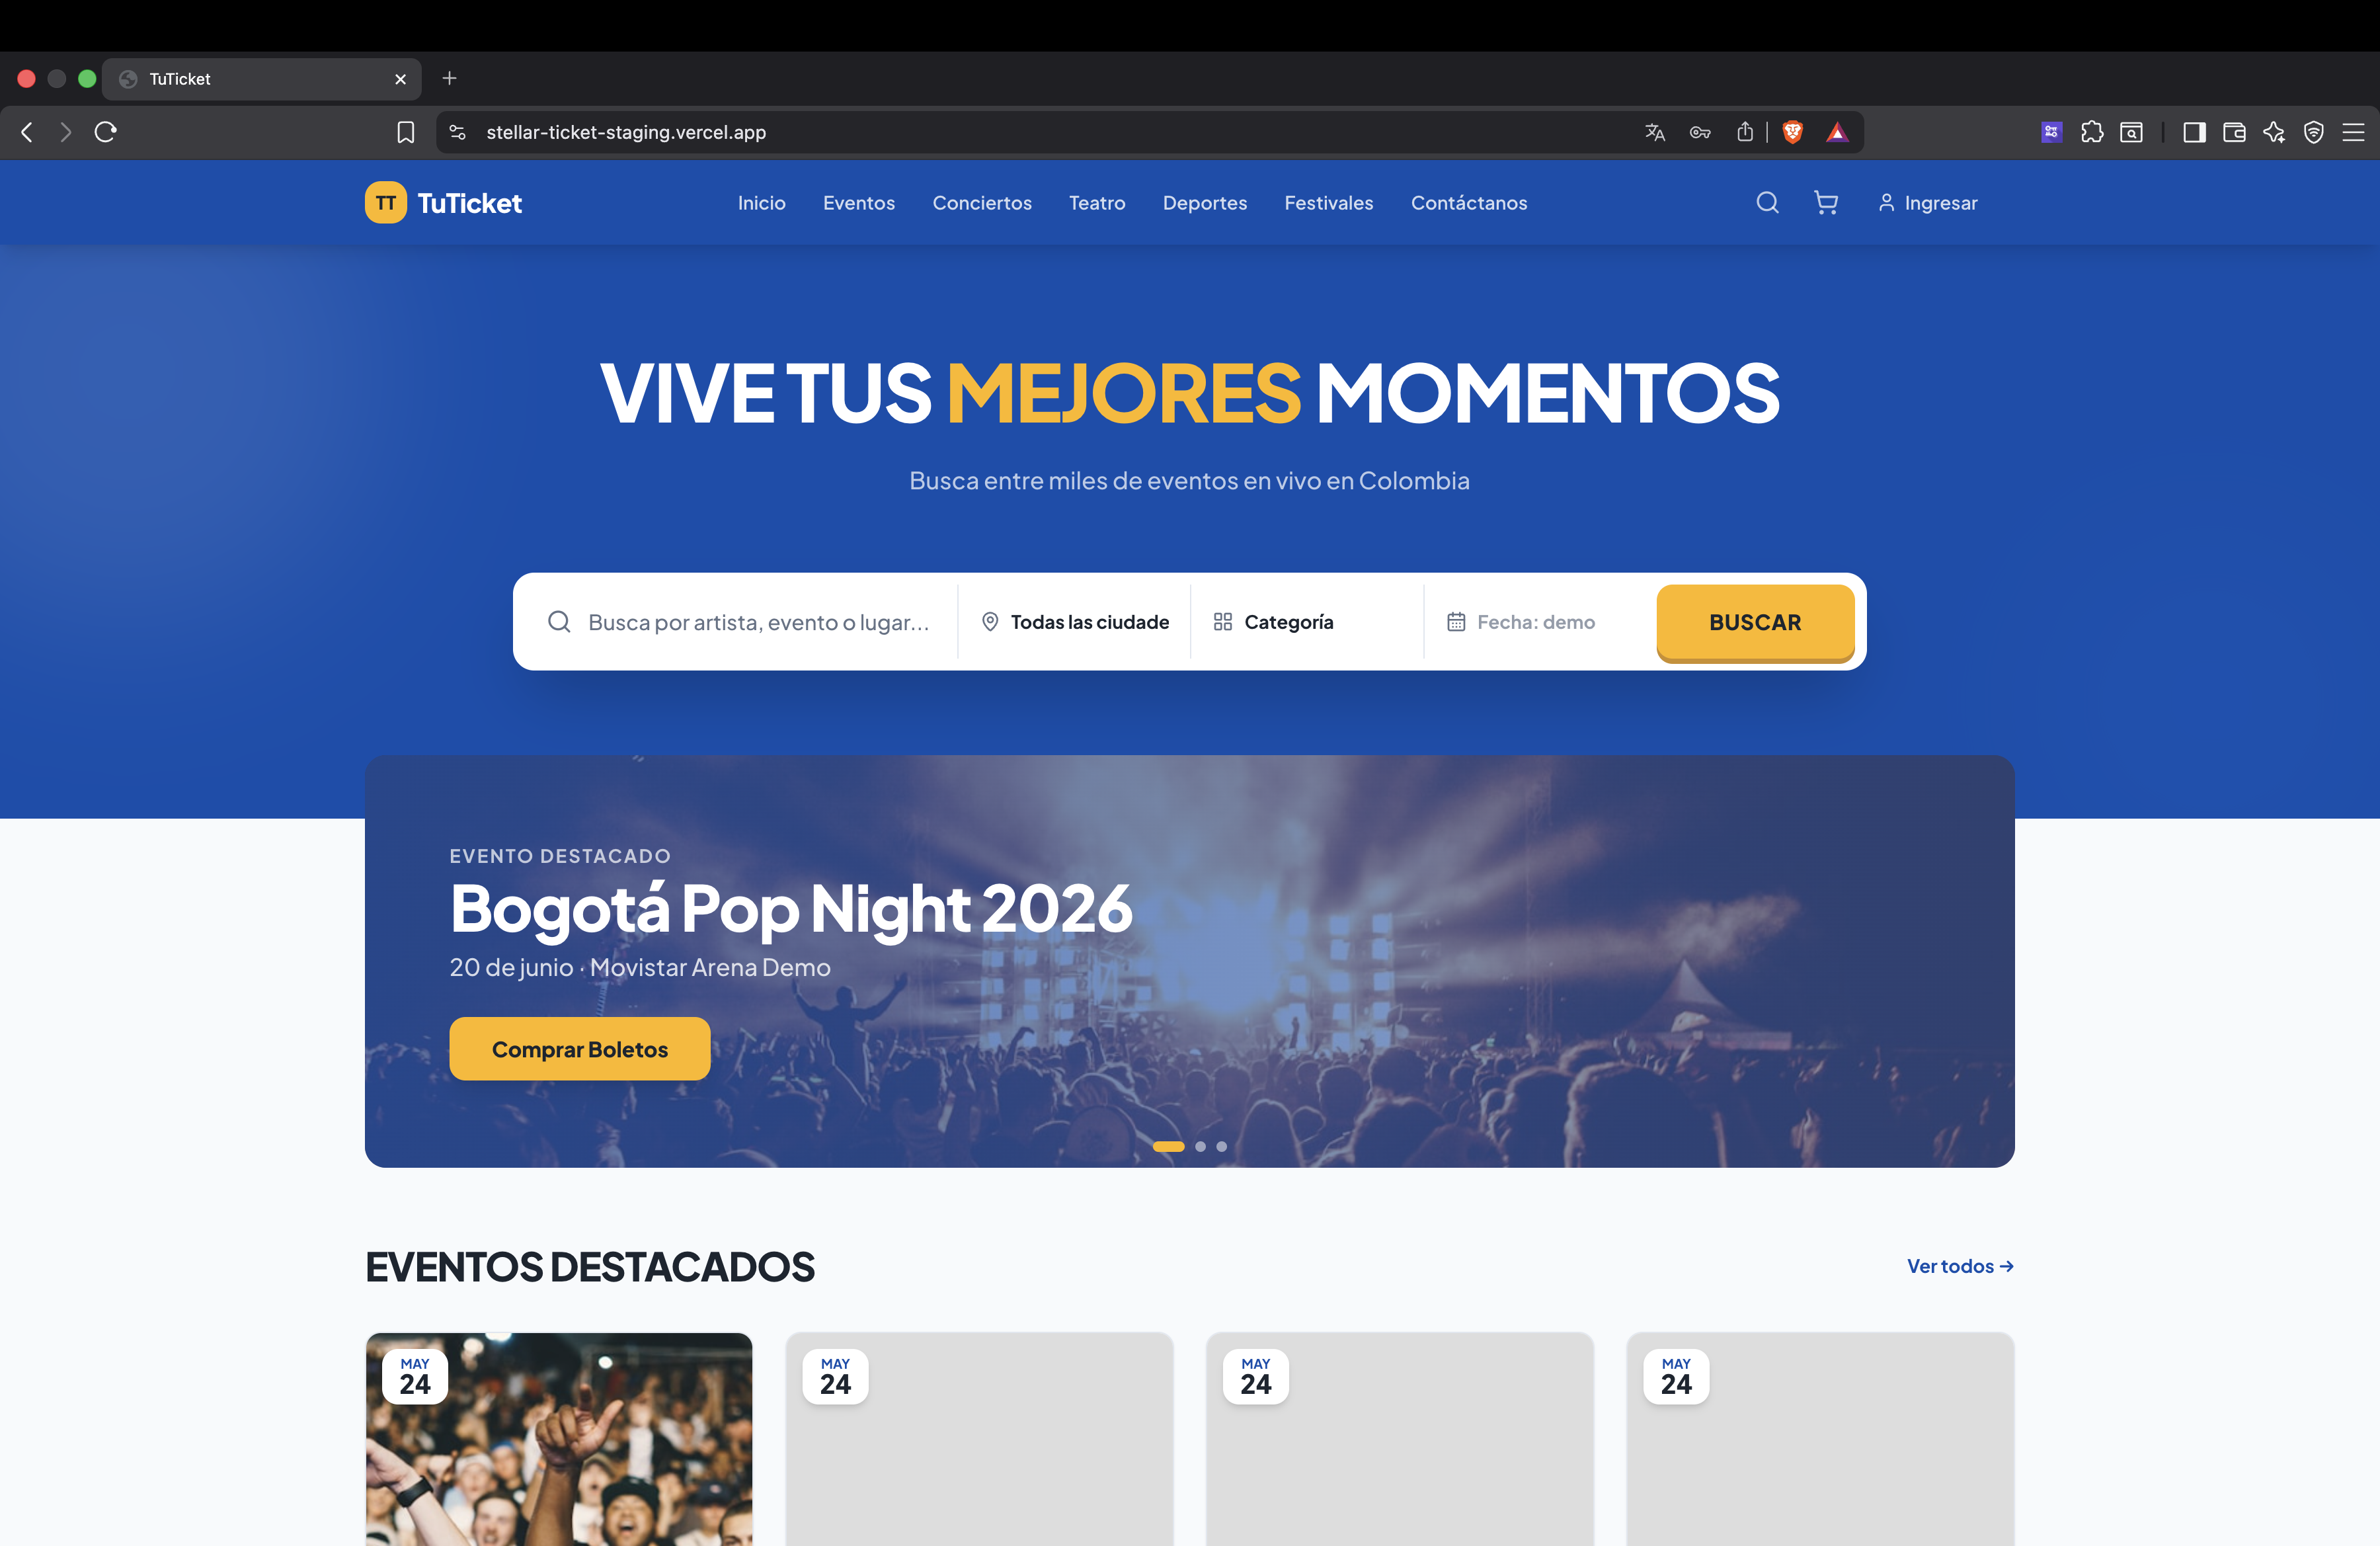
\includegraphics[width=0.92\textwidth]{Anexo/uat-01-acceso-sistema.png}
\caption{Evidencia UAT-01: acceso al sistema en ambiente de pruebas}
\label{fig:evidencia-uat-01}
\end{figure}

\begin{figure}[H]
\centering
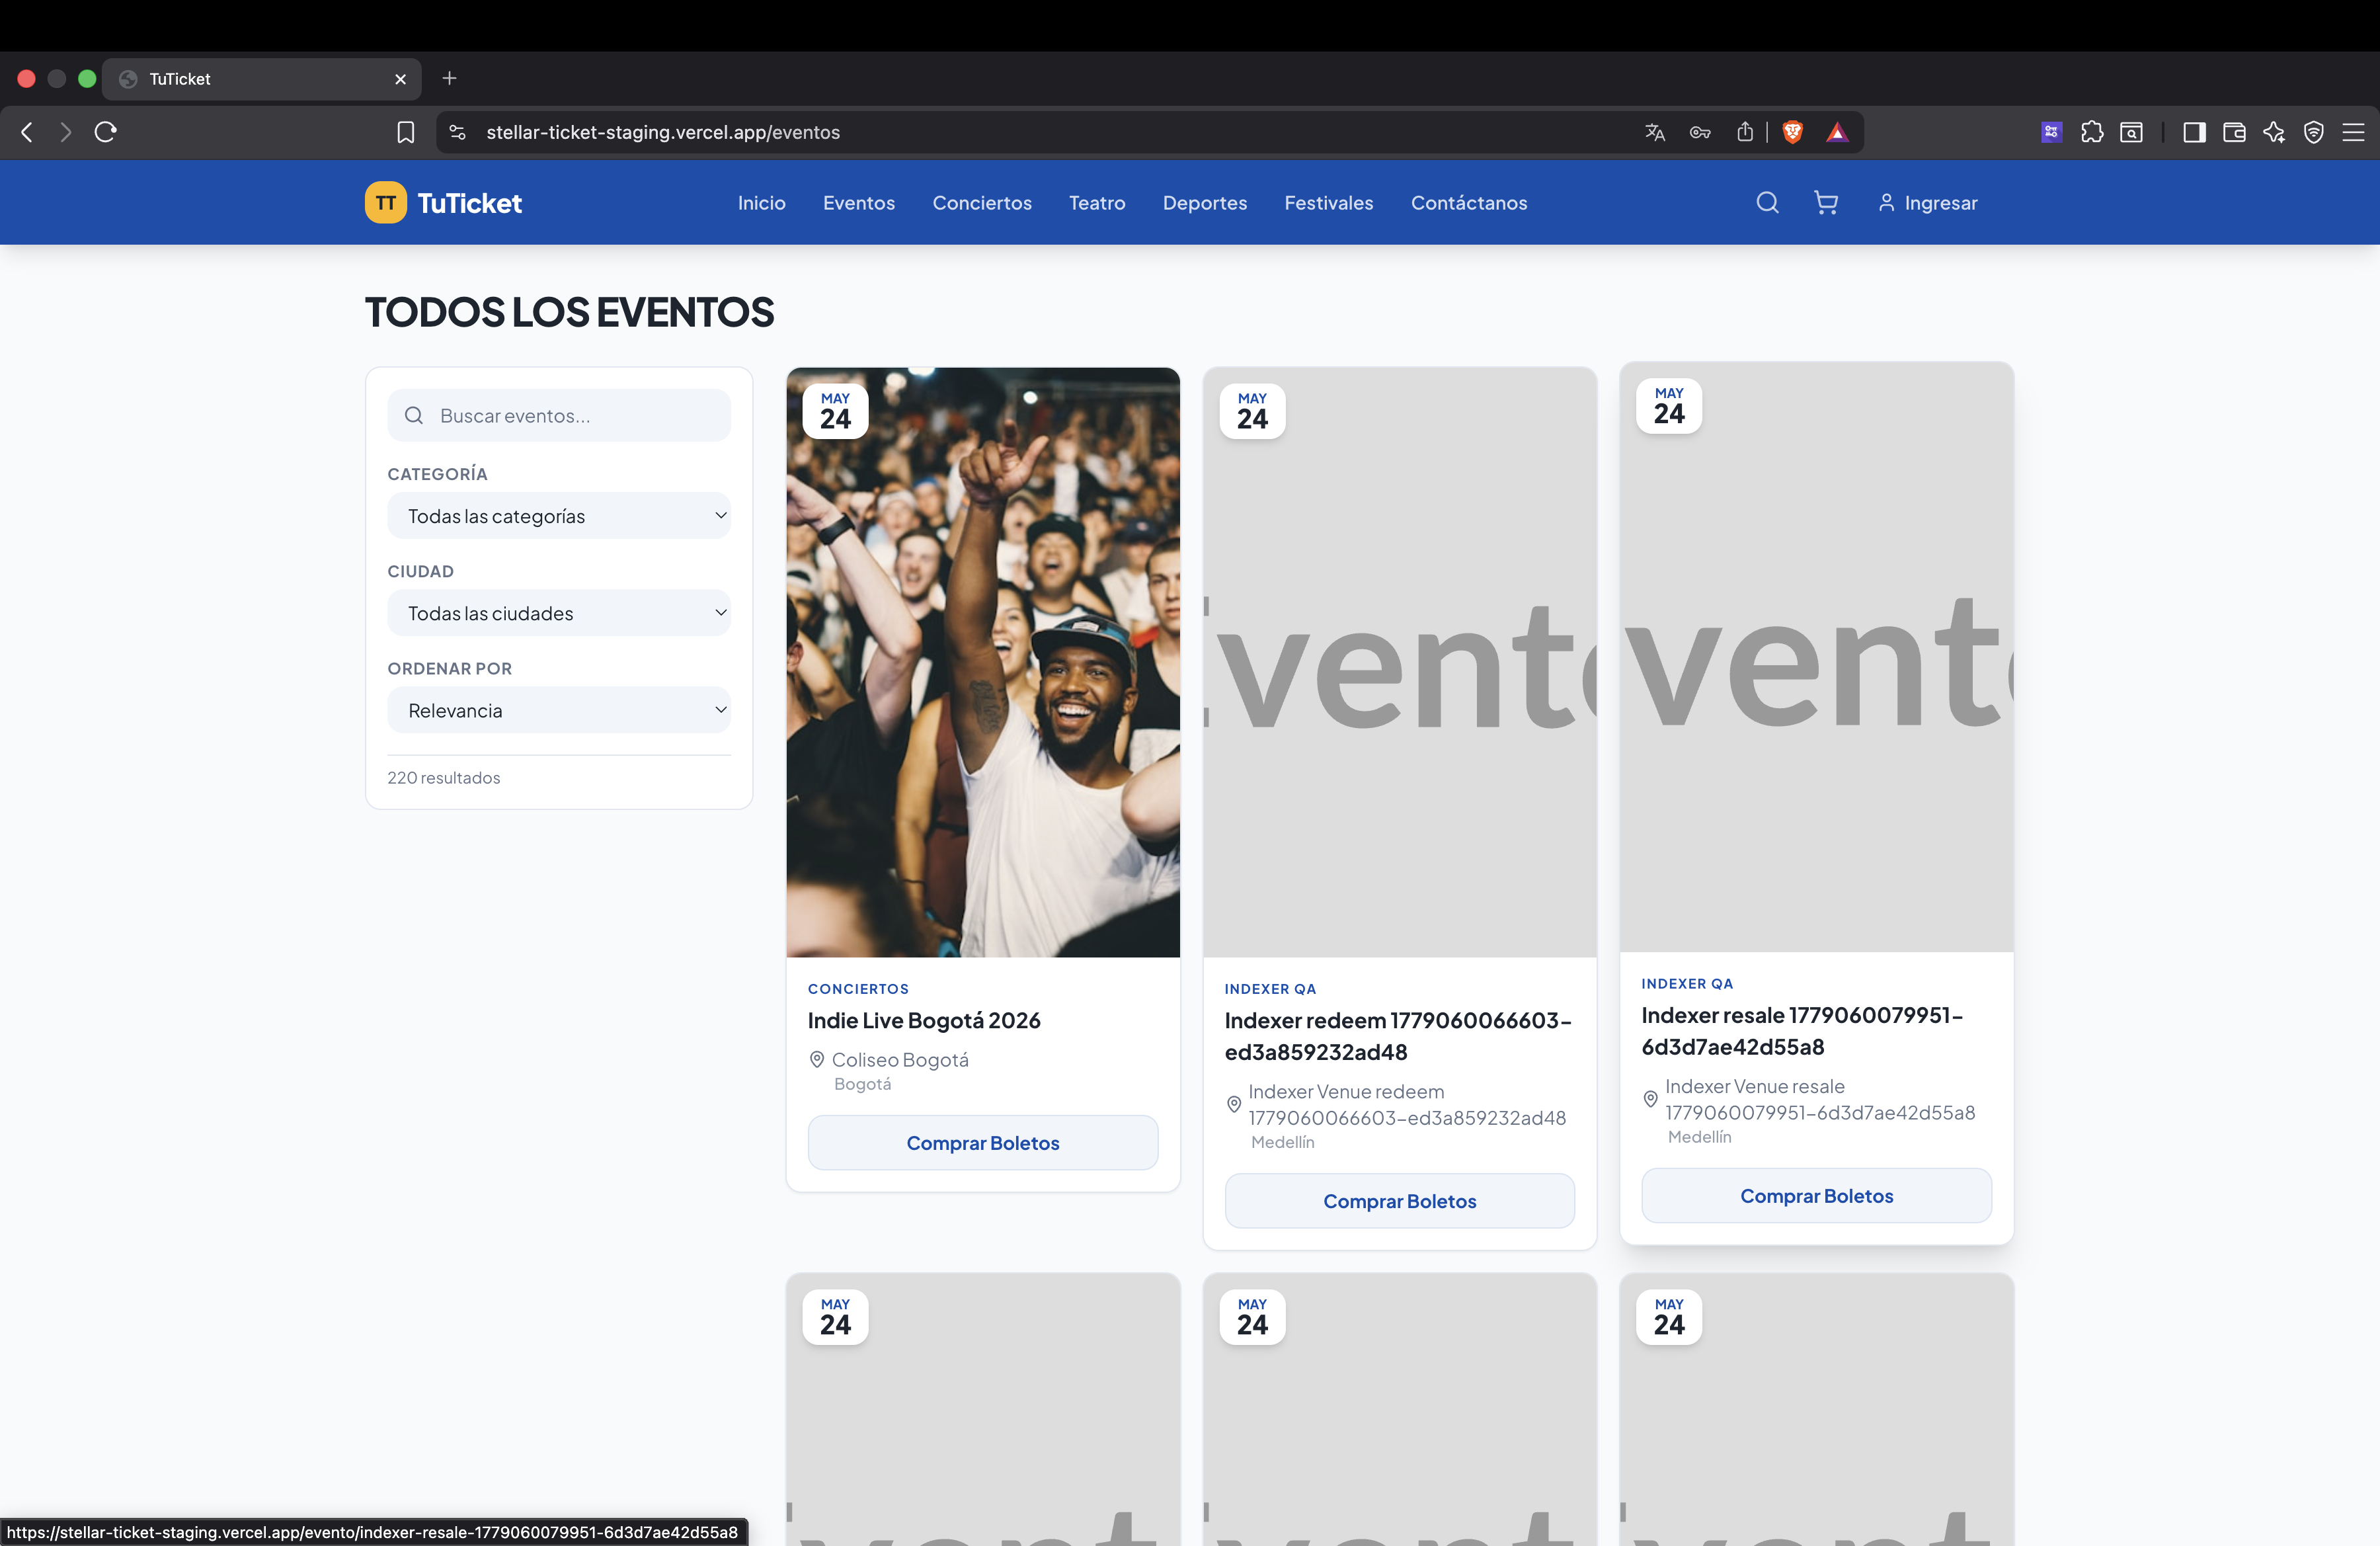
\includegraphics[width=0.92\textwidth]{Anexo/uat-02-consulta-eventos.png}
\caption{Evidencia UAT-02: consulta de eventos disponibles}
\label{fig:evidencia-uat-02}
\end{figure}

\begin{figure}[H]
\centering
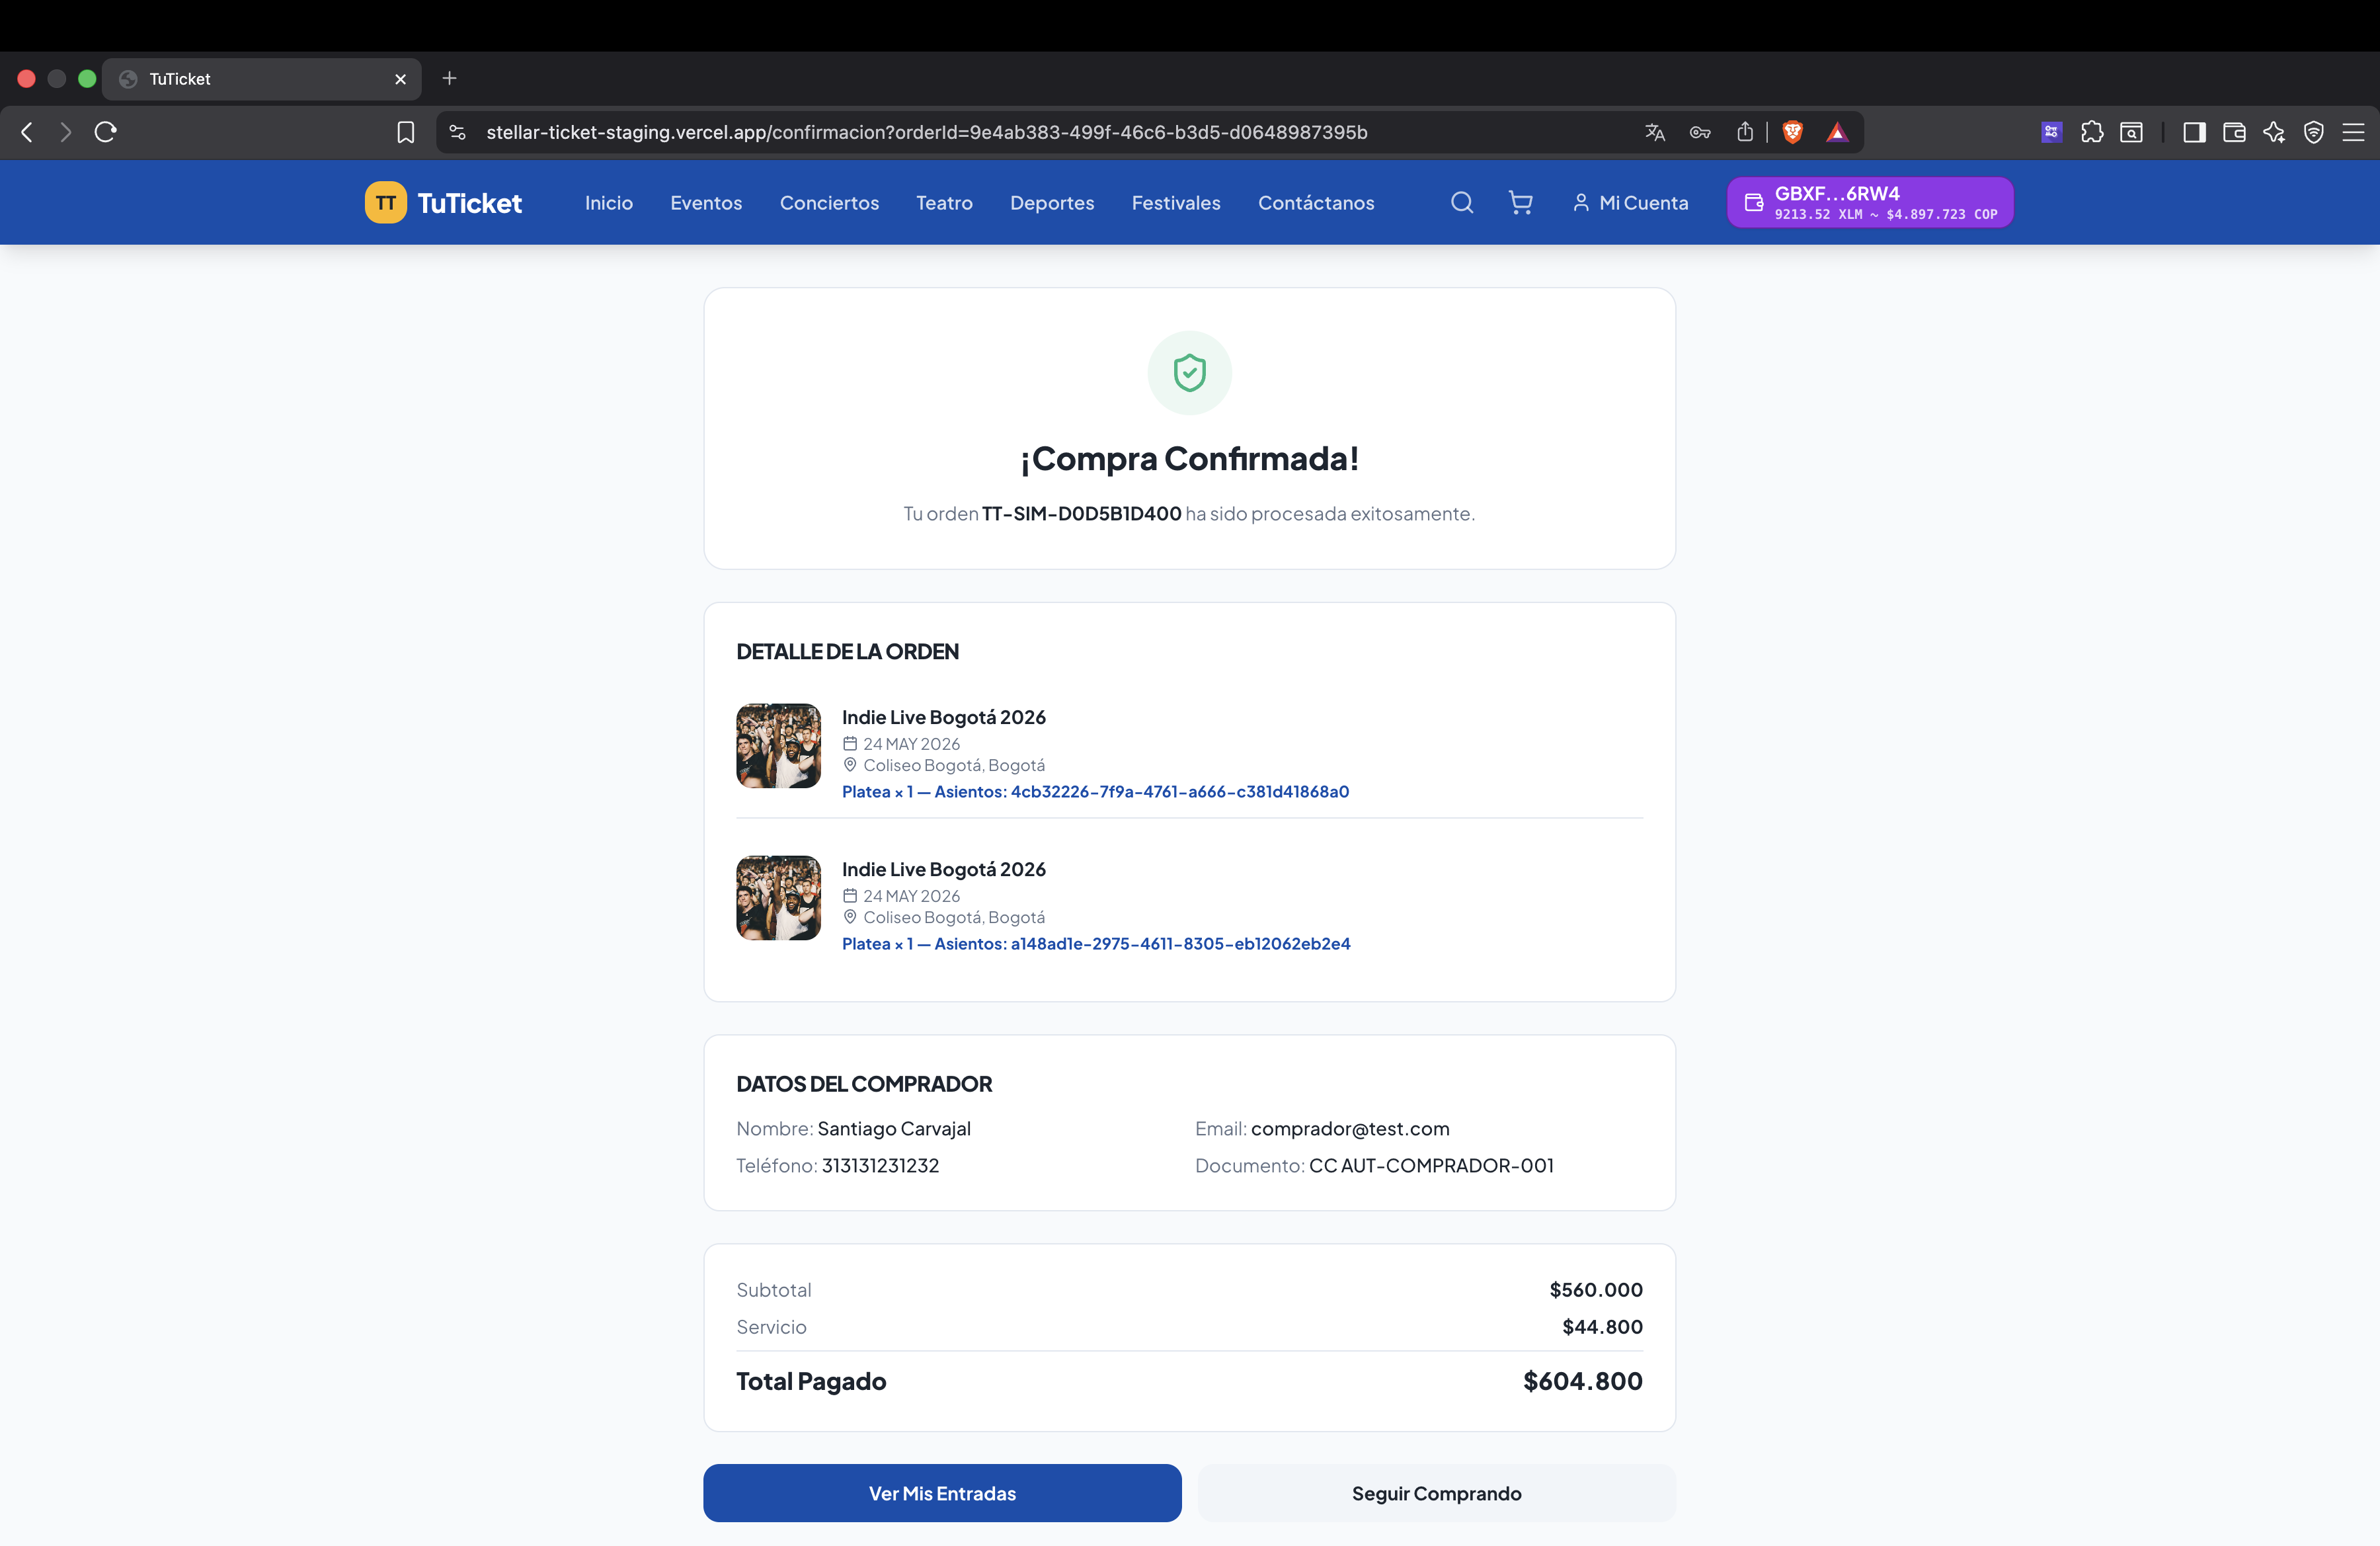
\includegraphics[width=0.92\textwidth]{Anexo/uat-03-compra-simulada.png}
\caption{Evidencia UAT-03: confirmación de compra primaria simulada}
\label{fig:evidencia-uat-03}
\end{figure}

\begin{figure}[H]
\centering
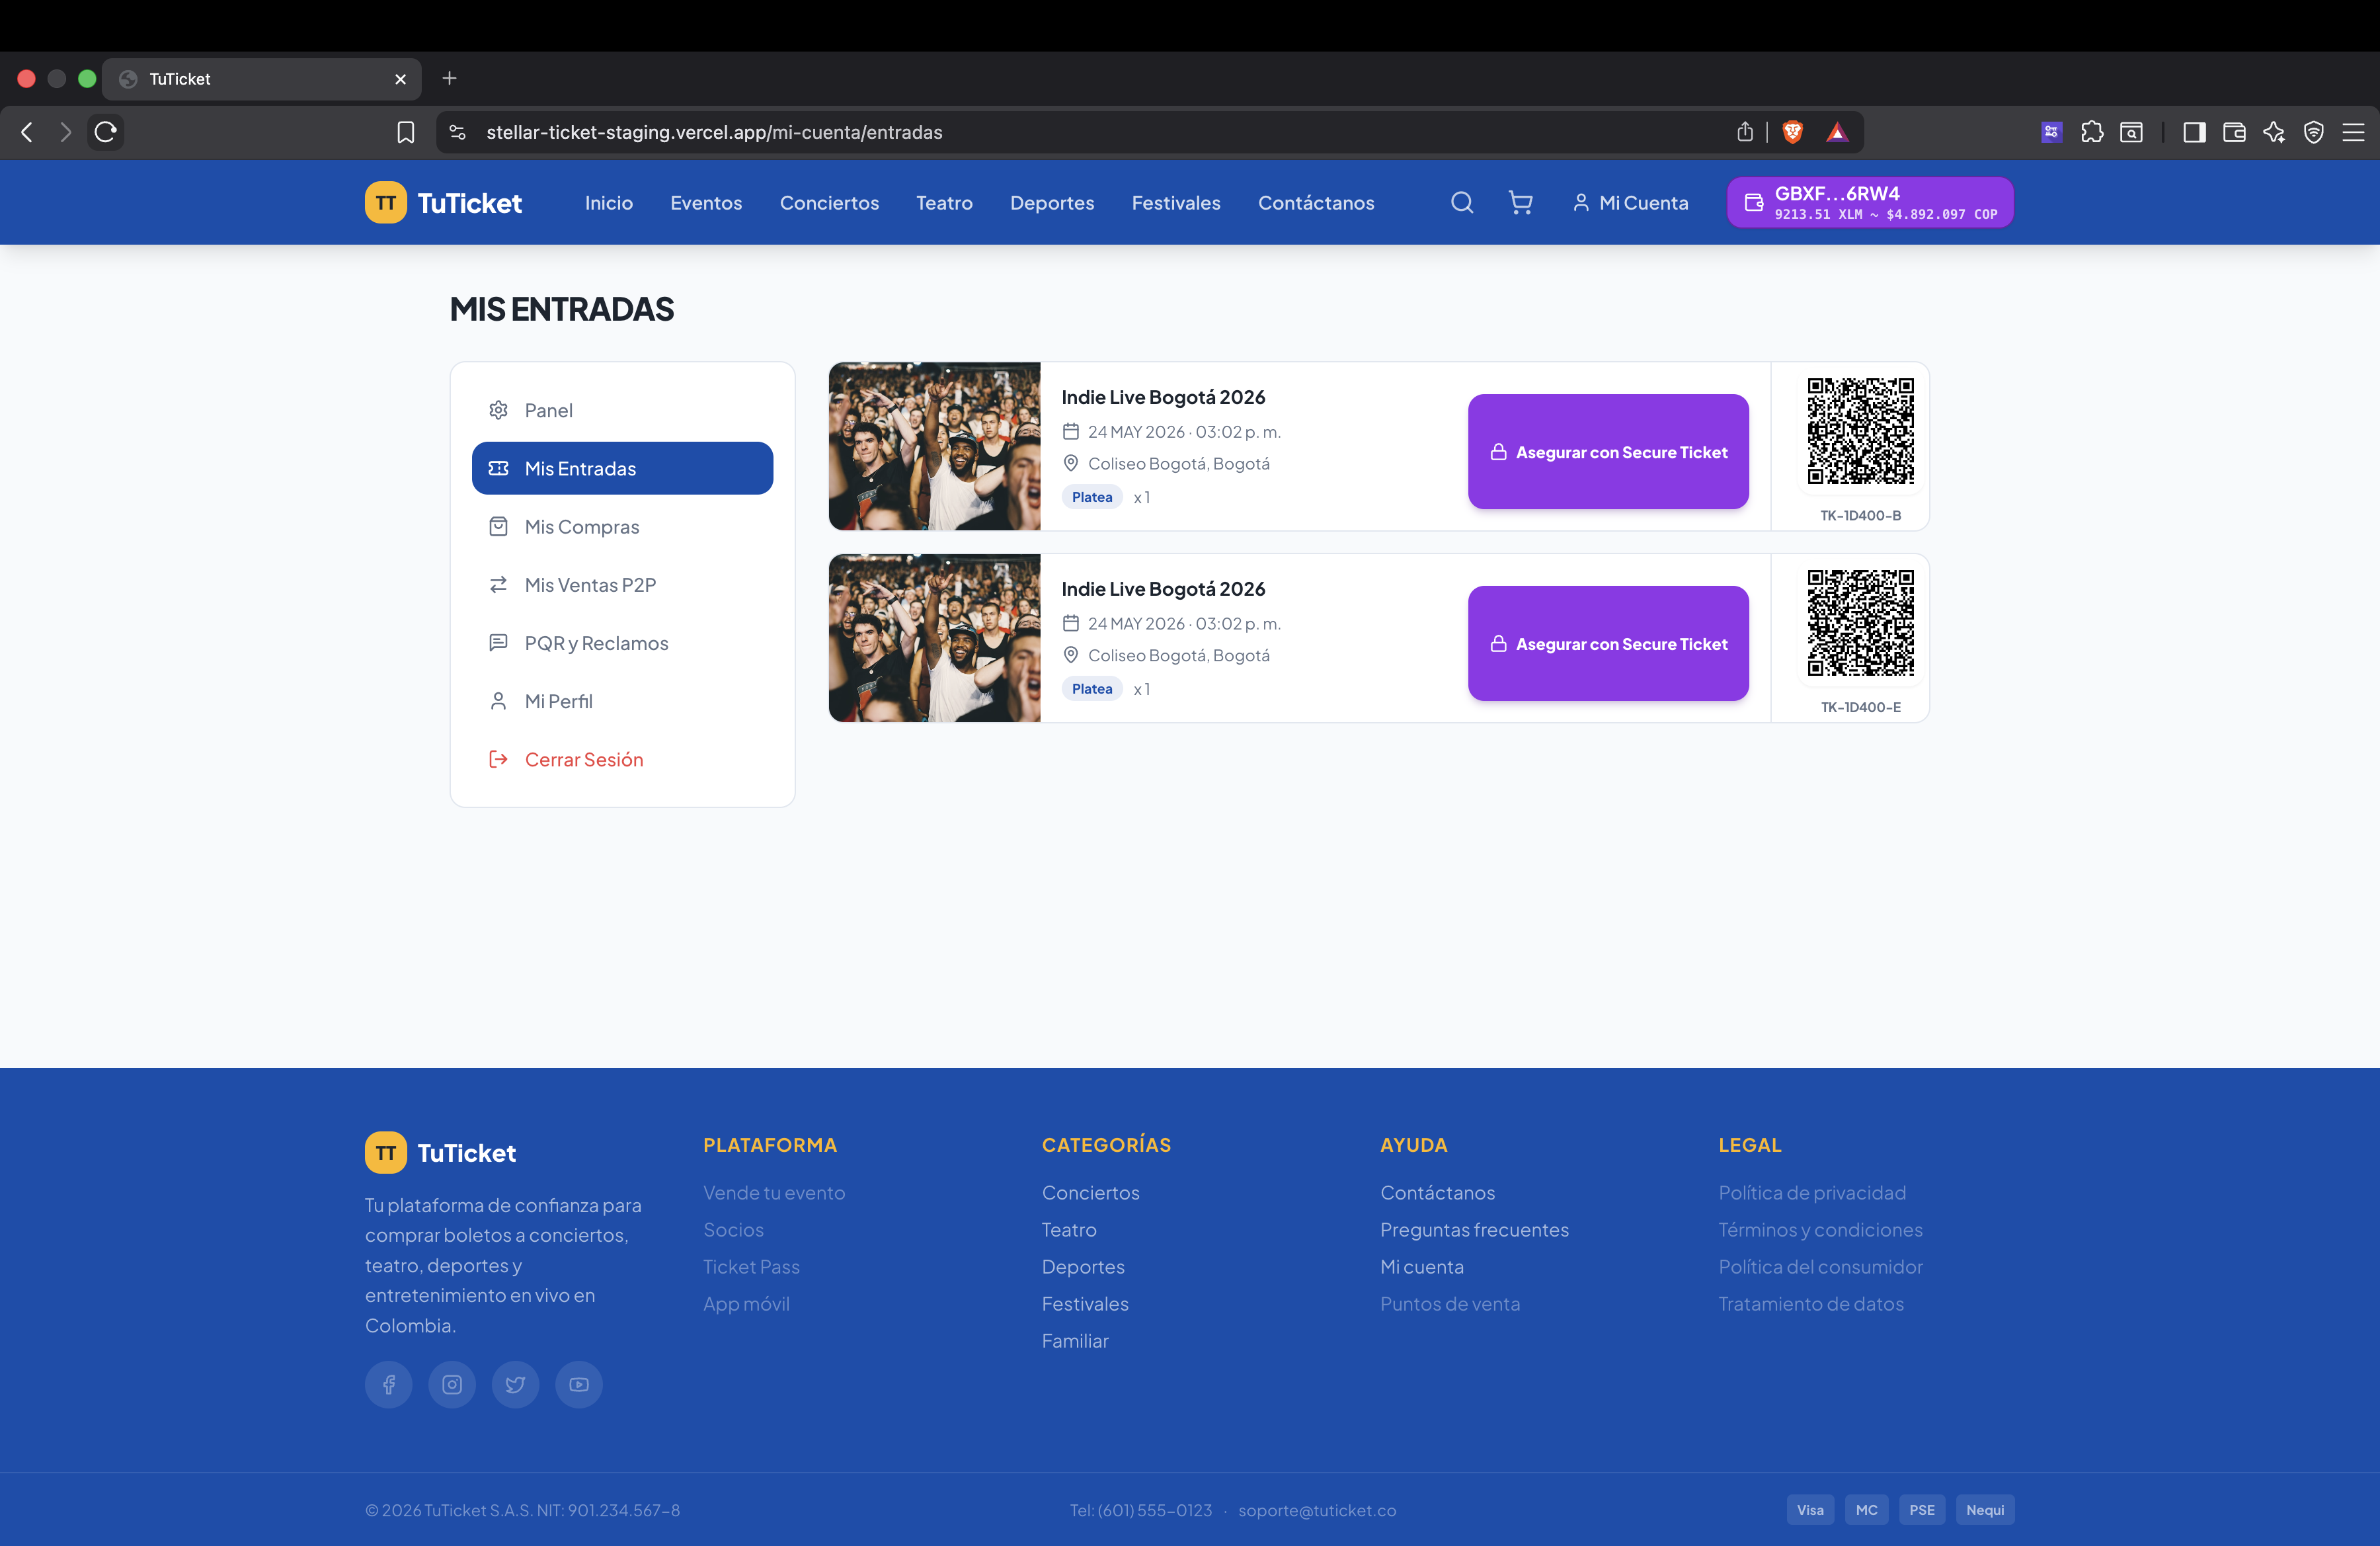
\includegraphics[width=0.92\textwidth]{Anexo/uat-04-inventario-tickets.png}
\caption{Evidencia UAT-04: consulta de inventario de tickets}
\label{fig:evidencia-uat-04}
\end{figure}

\begin{figure}[H]
\centering
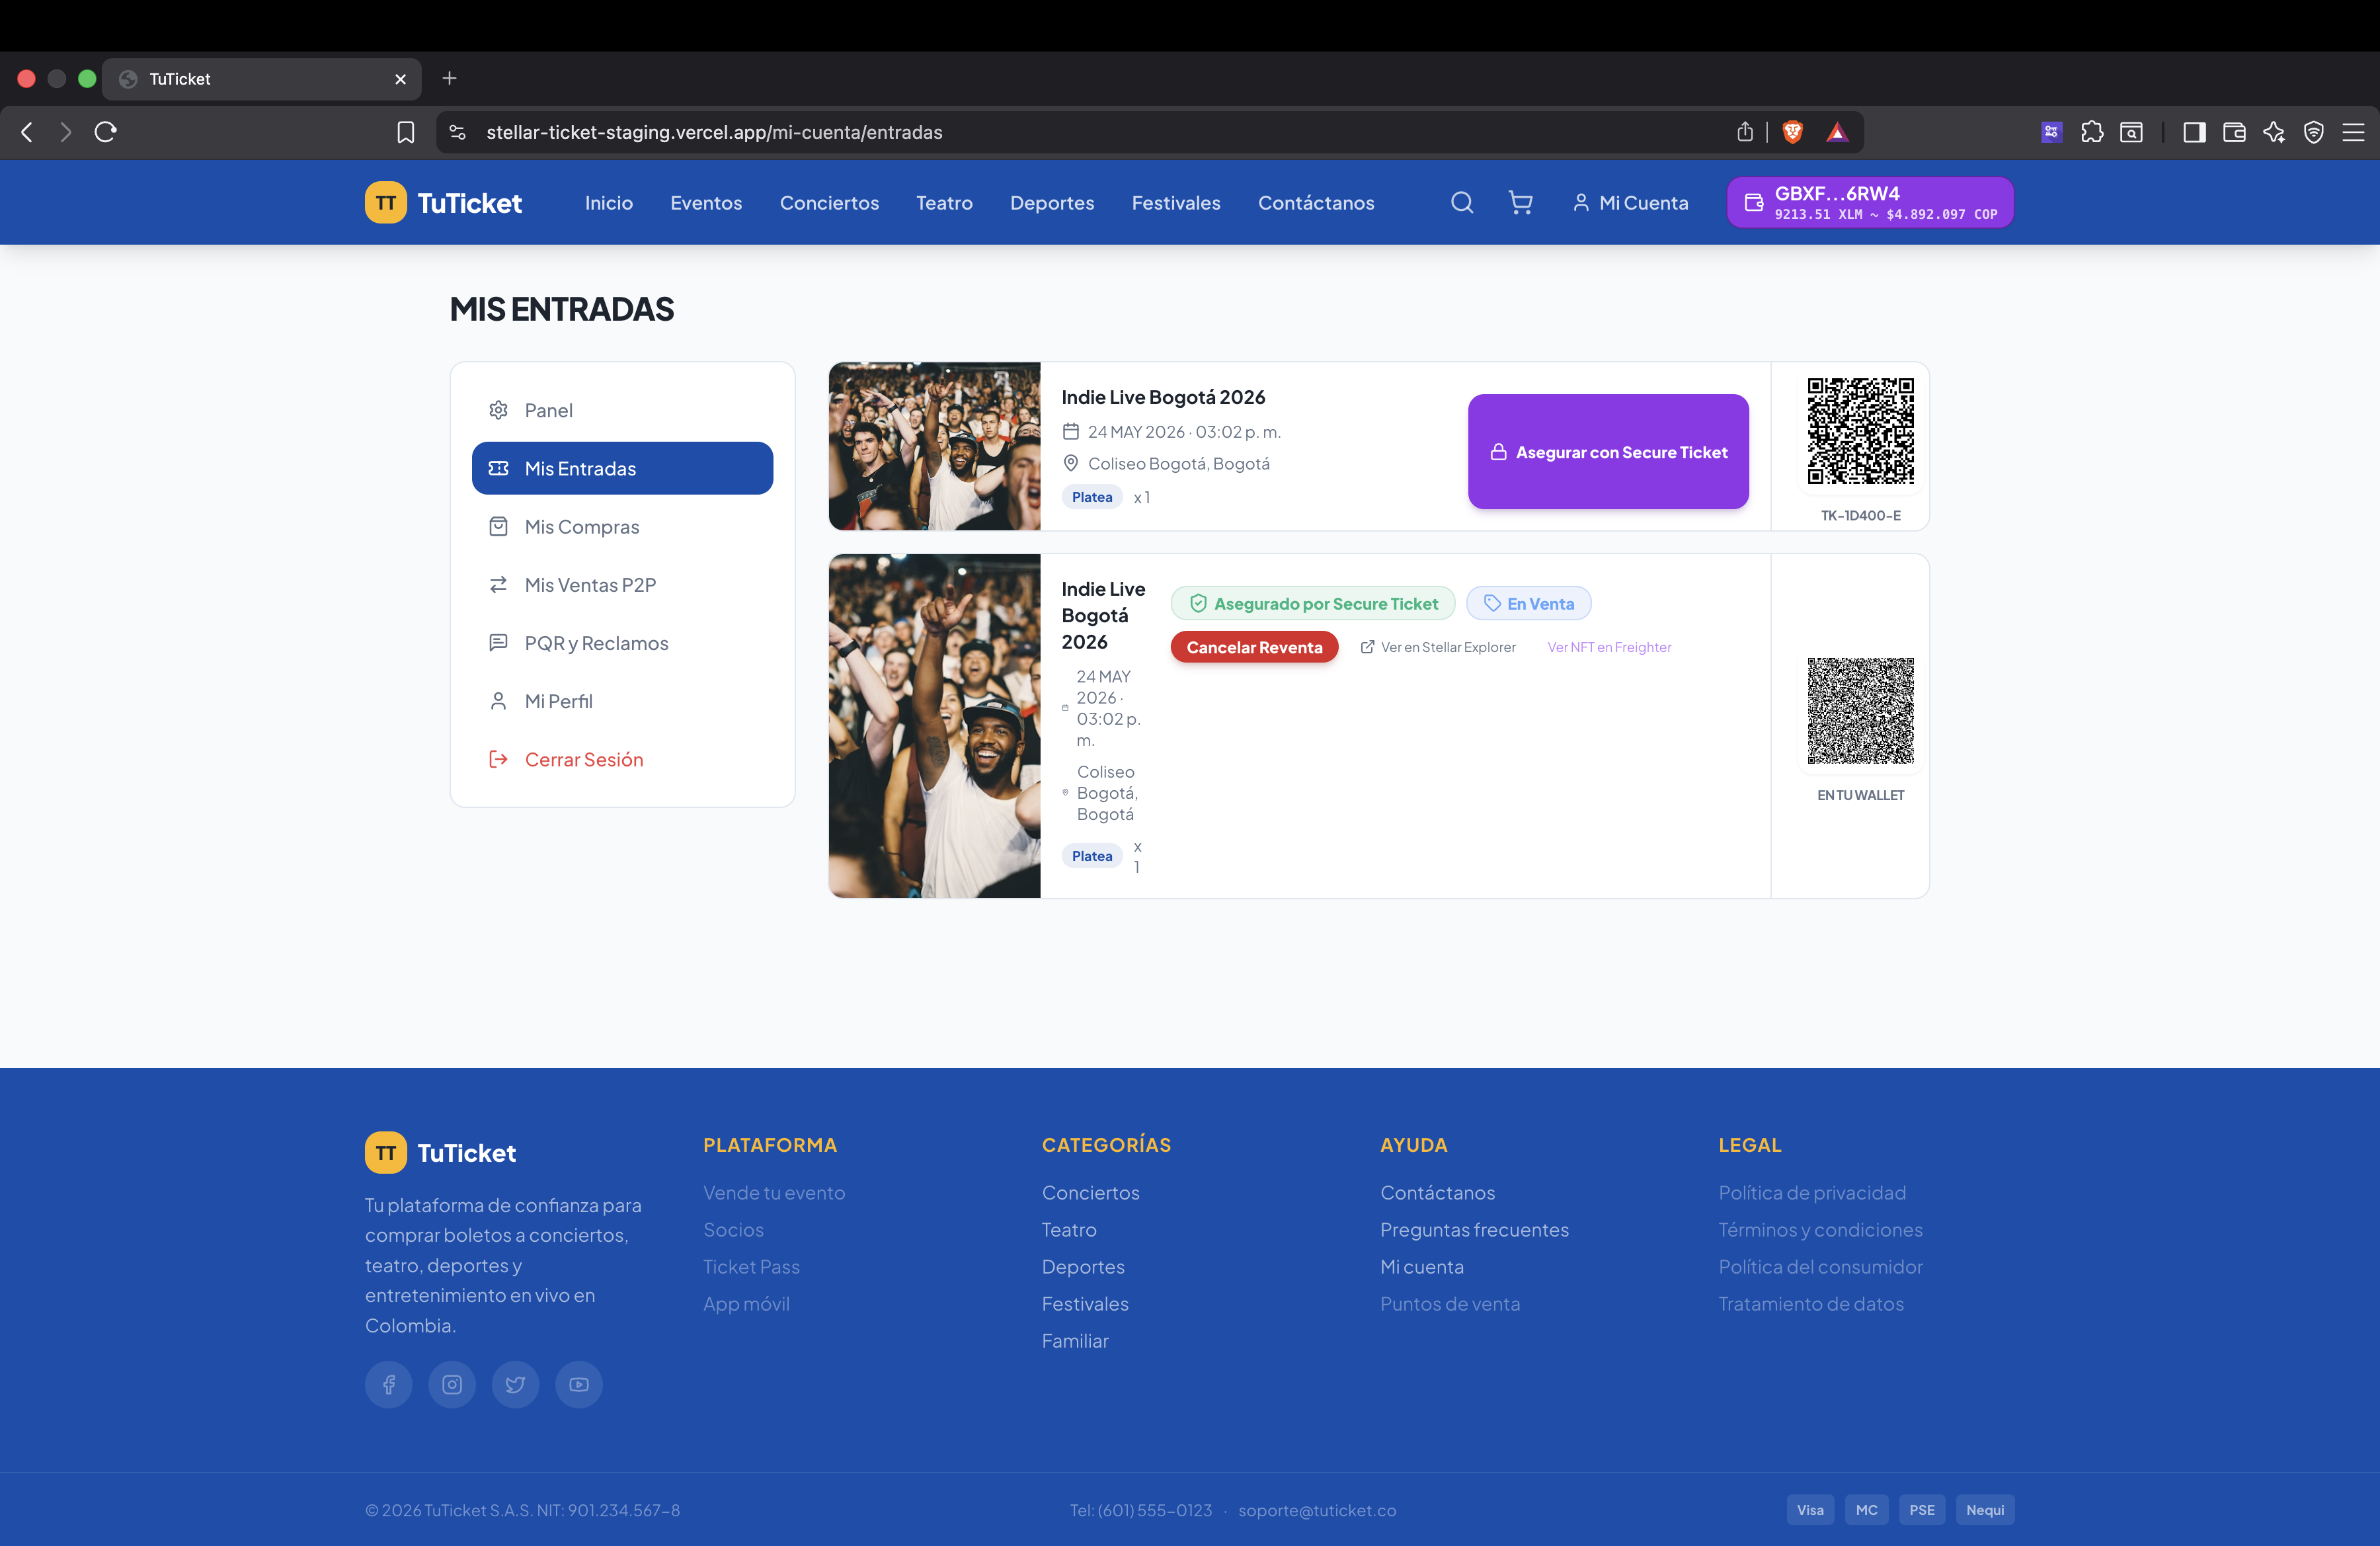
\includegraphics[width=0.92\textwidth]{Anexo/uat-05-publicacion-reventa.png}
\caption{Evidencia UAT-05: publicación de ticket para reventa}
\label{fig:evidencia-uat-05}
\end{figure}

\begin{figure}[H]
\centering
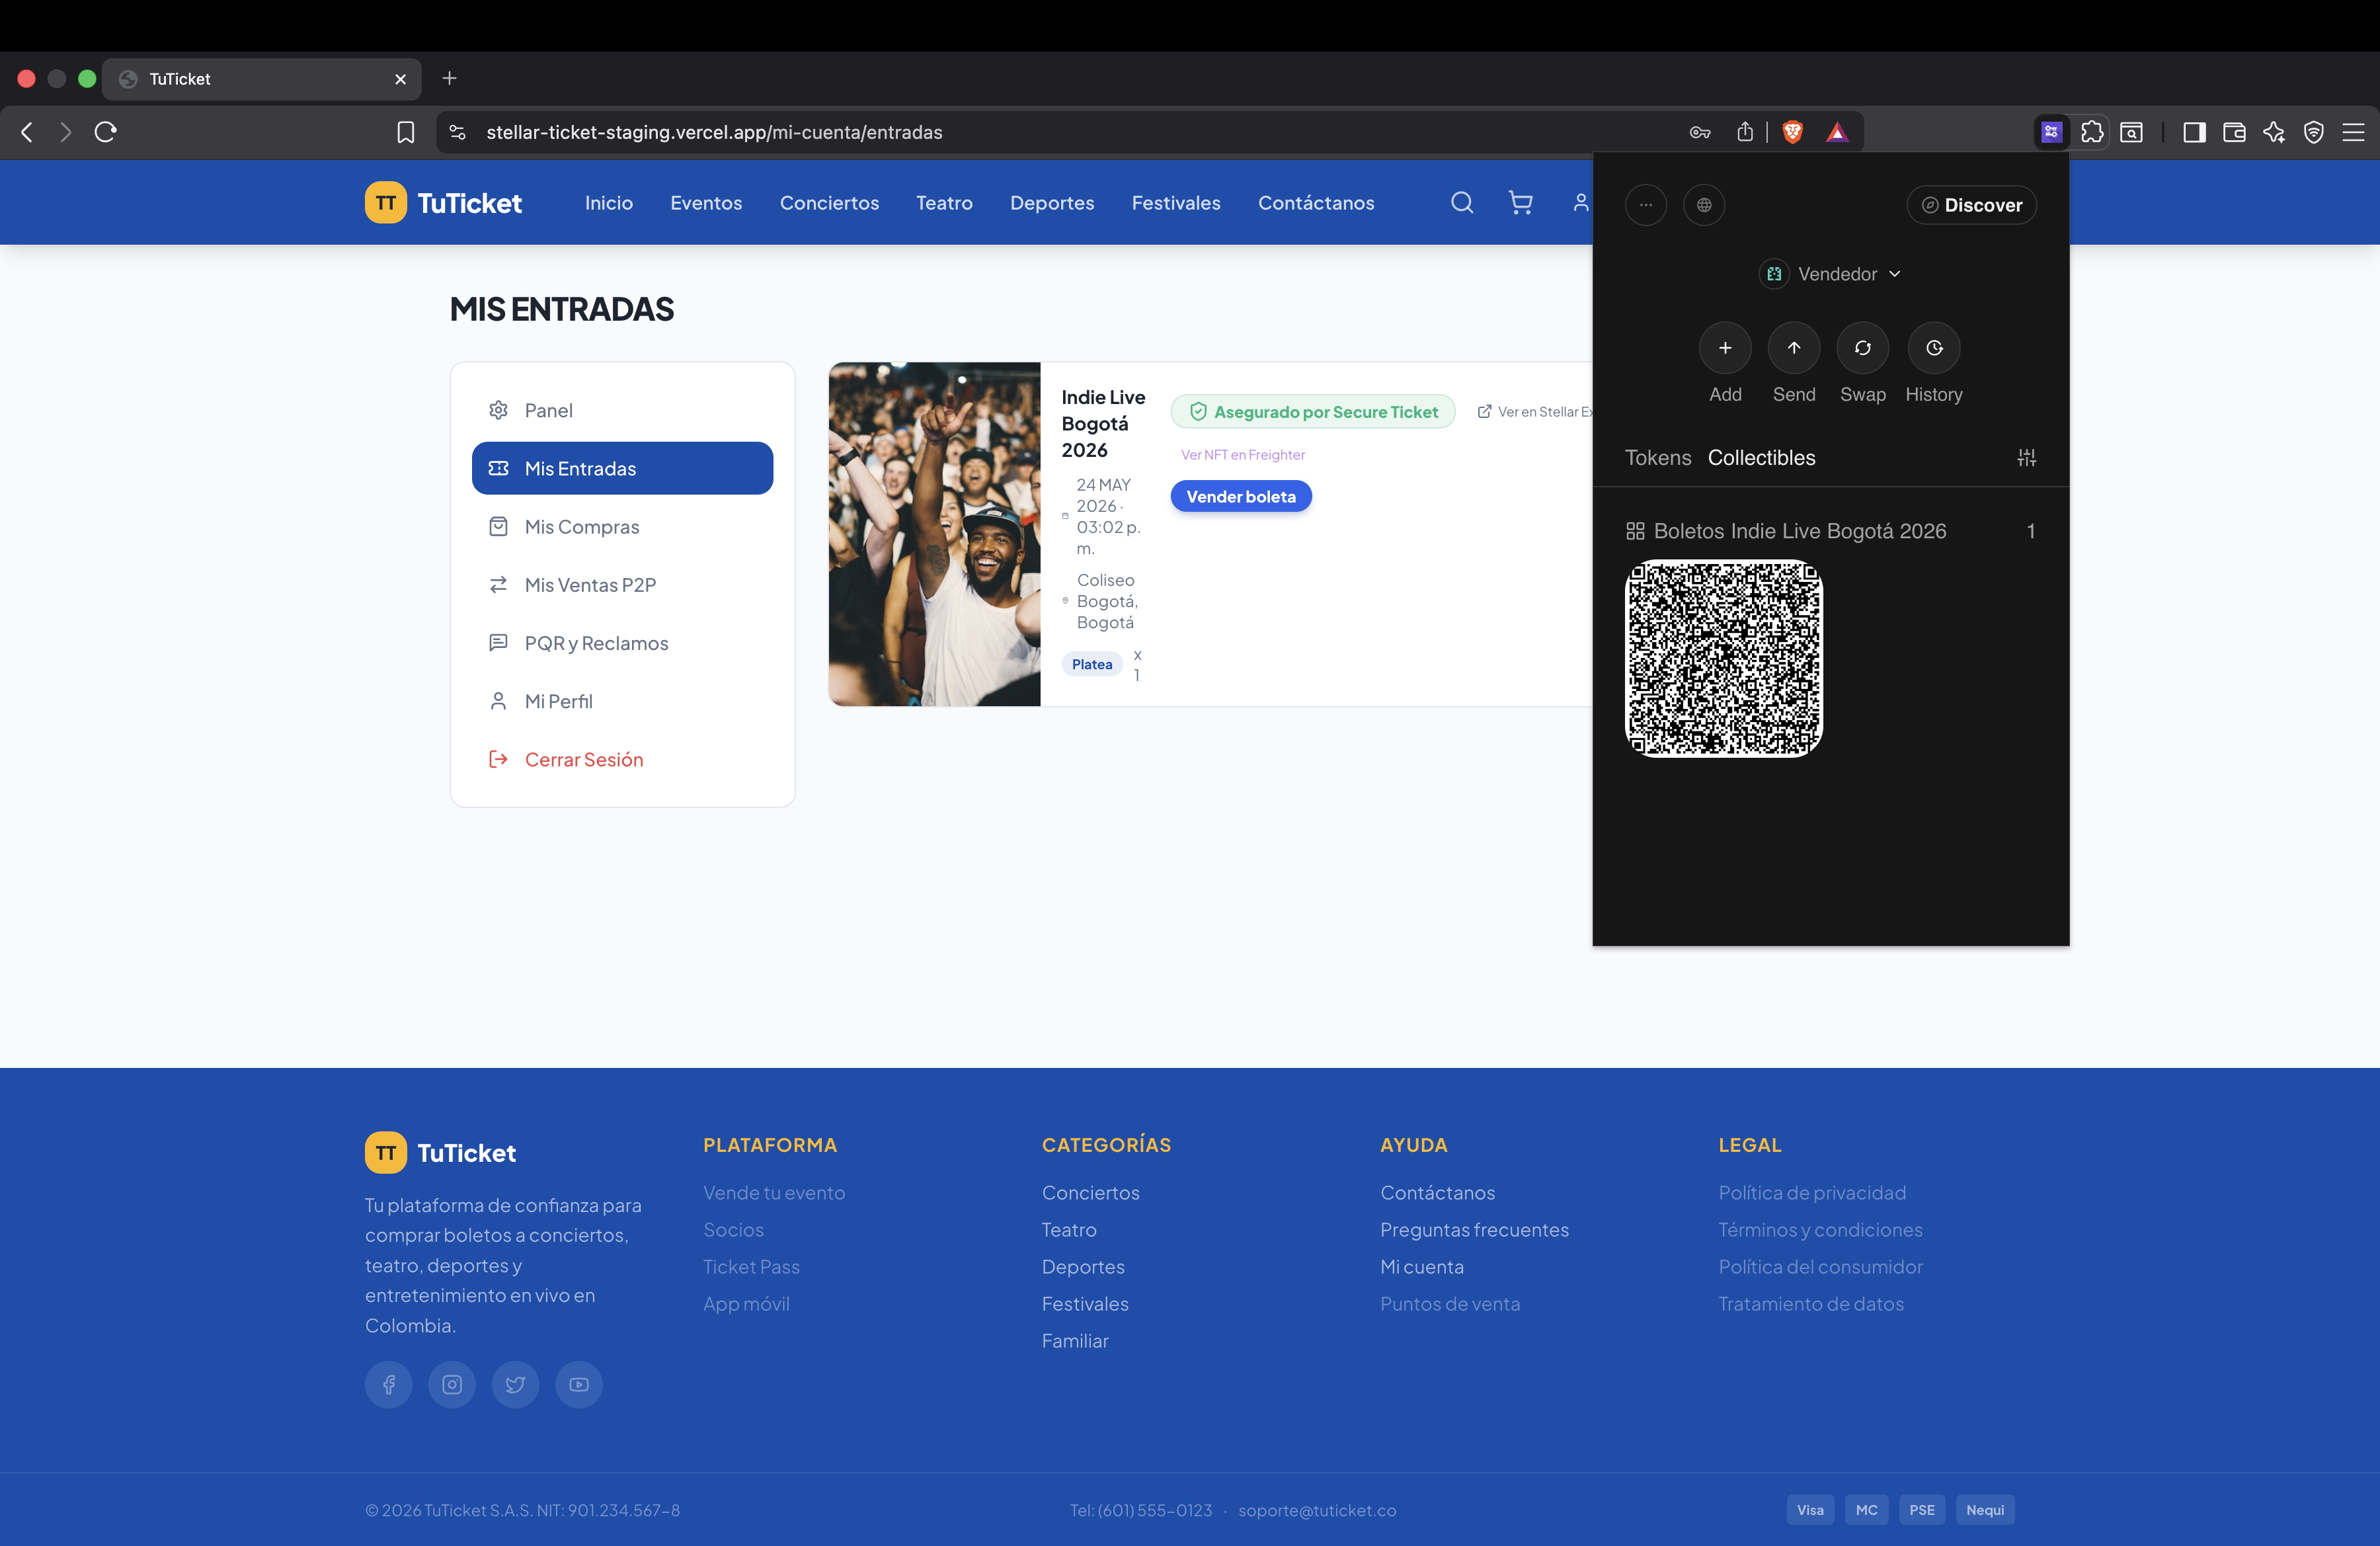
\includegraphics[width=0.92\textwidth]{Anexo/uat-06-compra-reventa.png}
\caption{Evidencia UAT-06: soporte visual del flujo de reventa bajo datos preparados}
\label{fig:evidencia-uat-06}
\end{figure}

\begin{figure}[H]
\centering
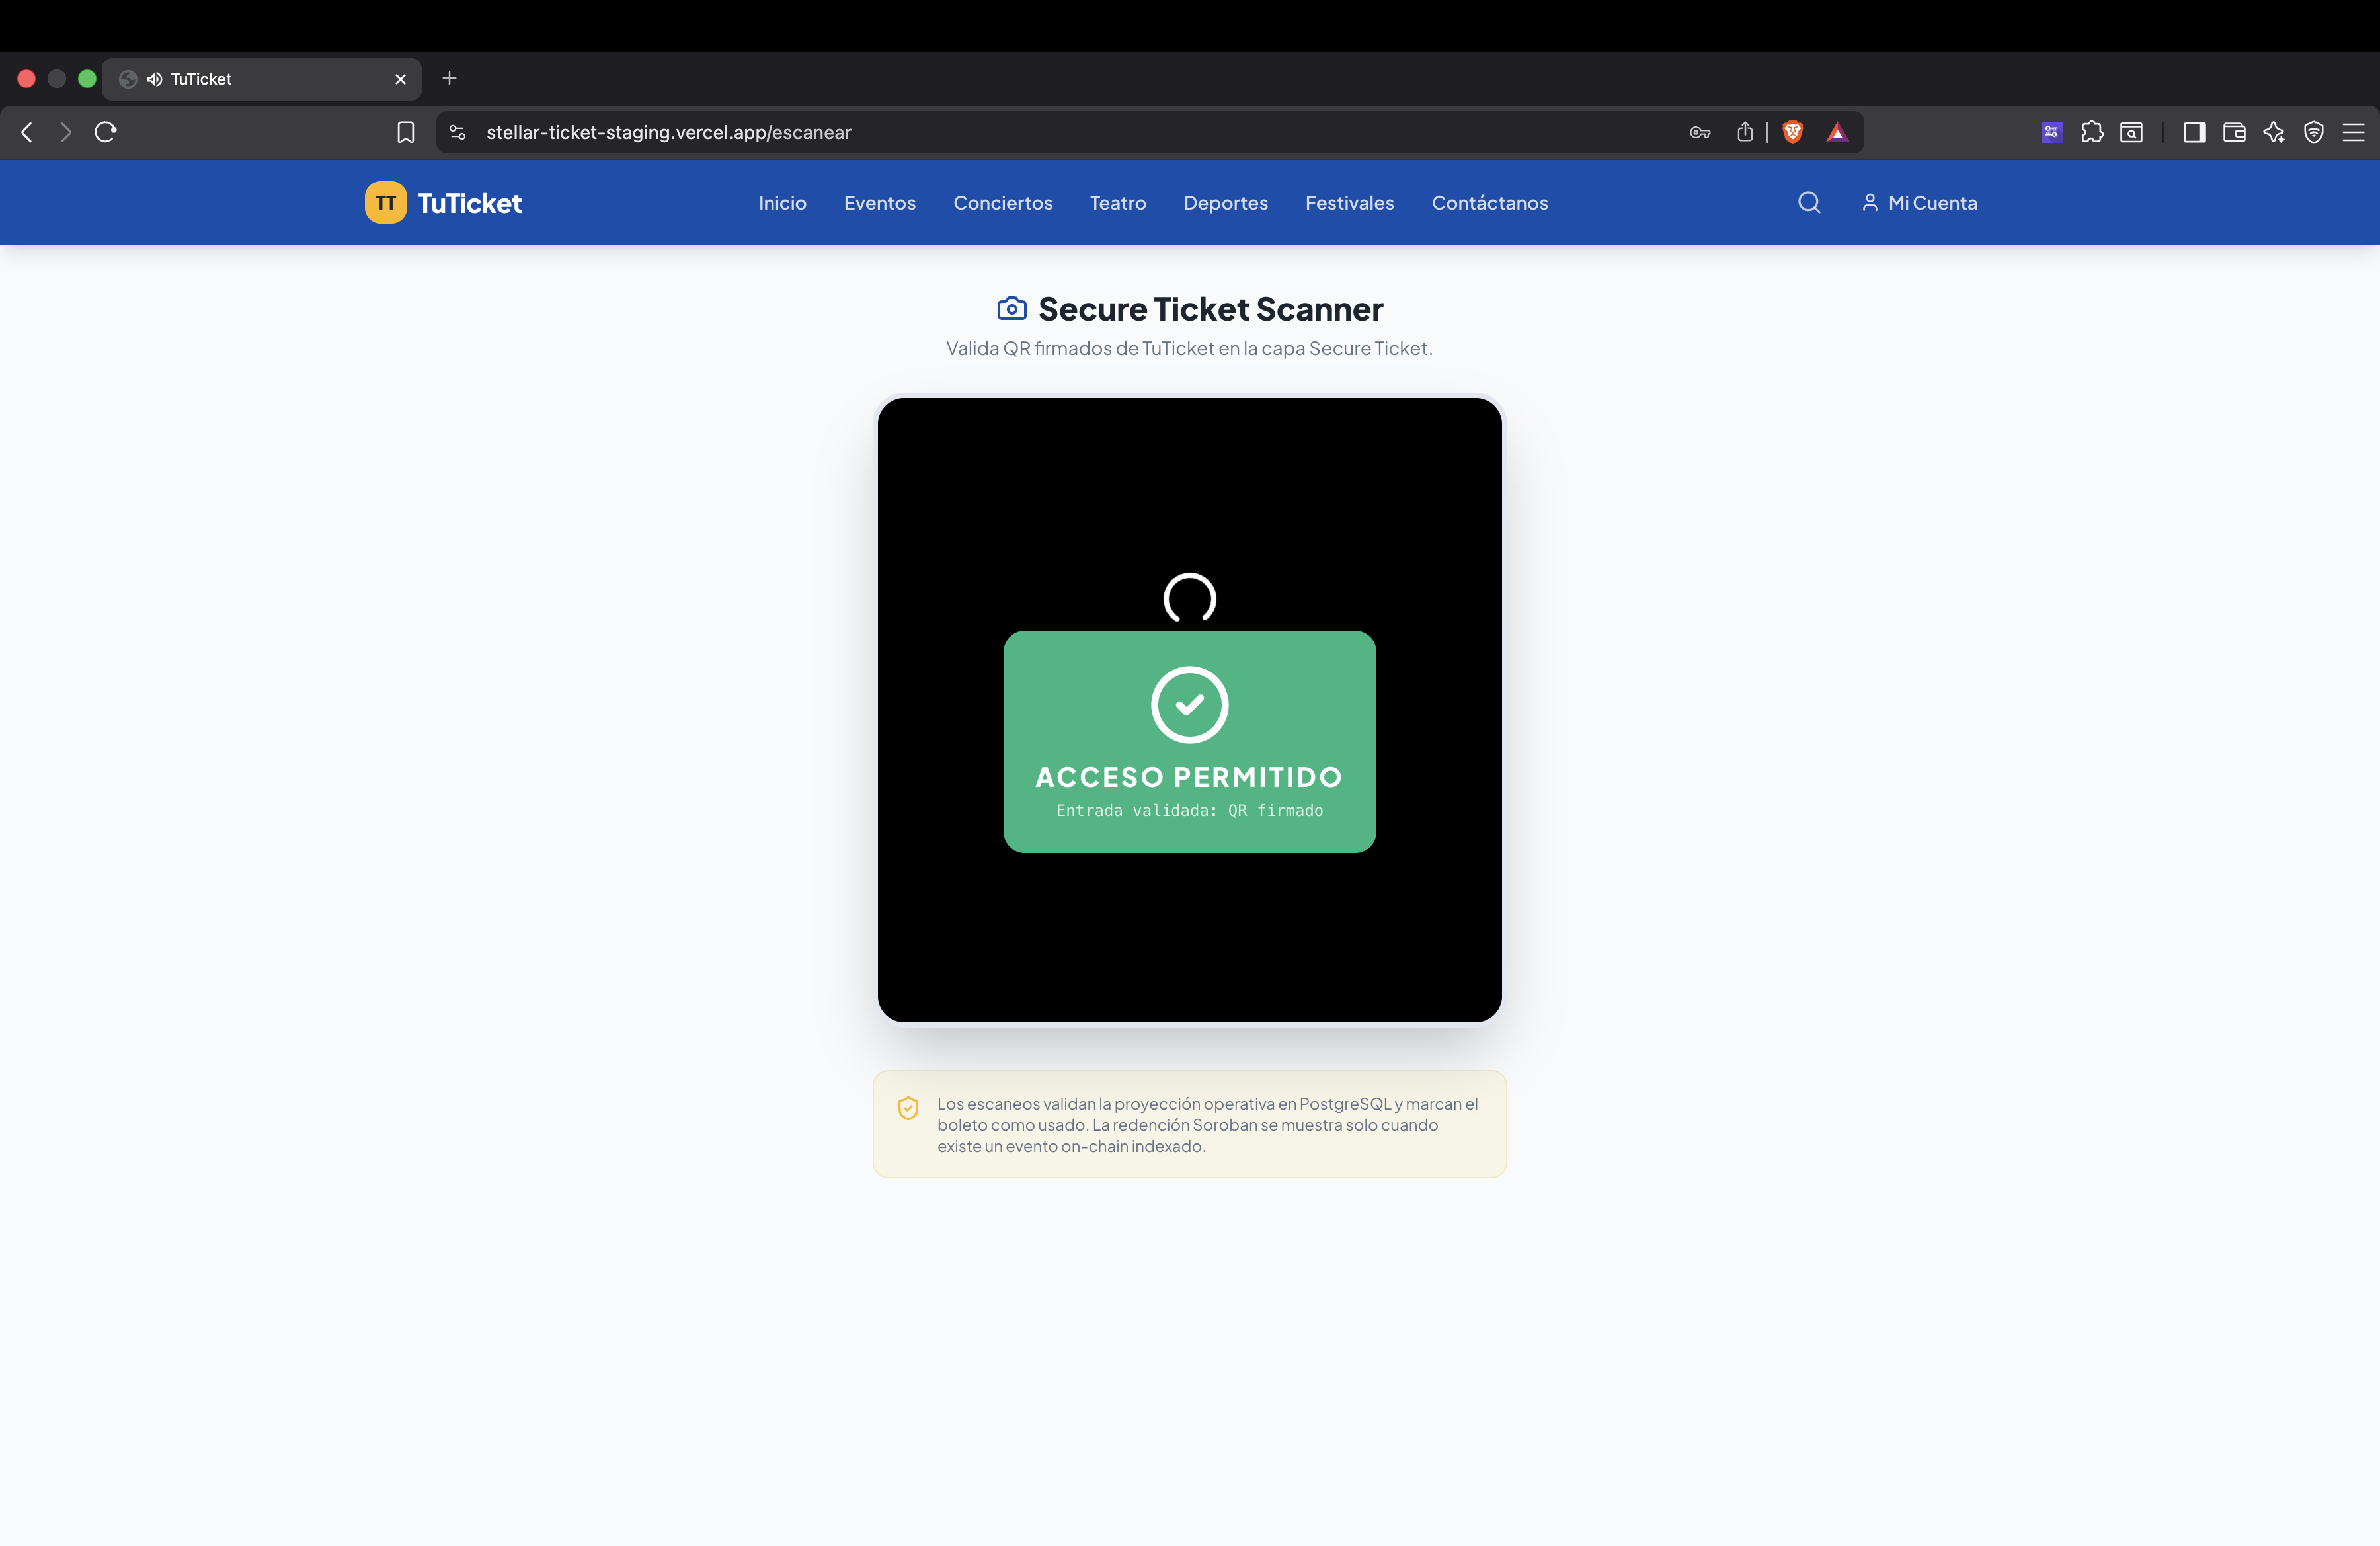
\includegraphics[width=0.92\textwidth]{Anexo/uat-07-verificacion-qr.png}
\caption{Evidencia UAT-07: verificación exitosa mediante QR}
\label{fig:evidencia-uat-07}
\end{figure}

\begin{figure}[H]
\centering
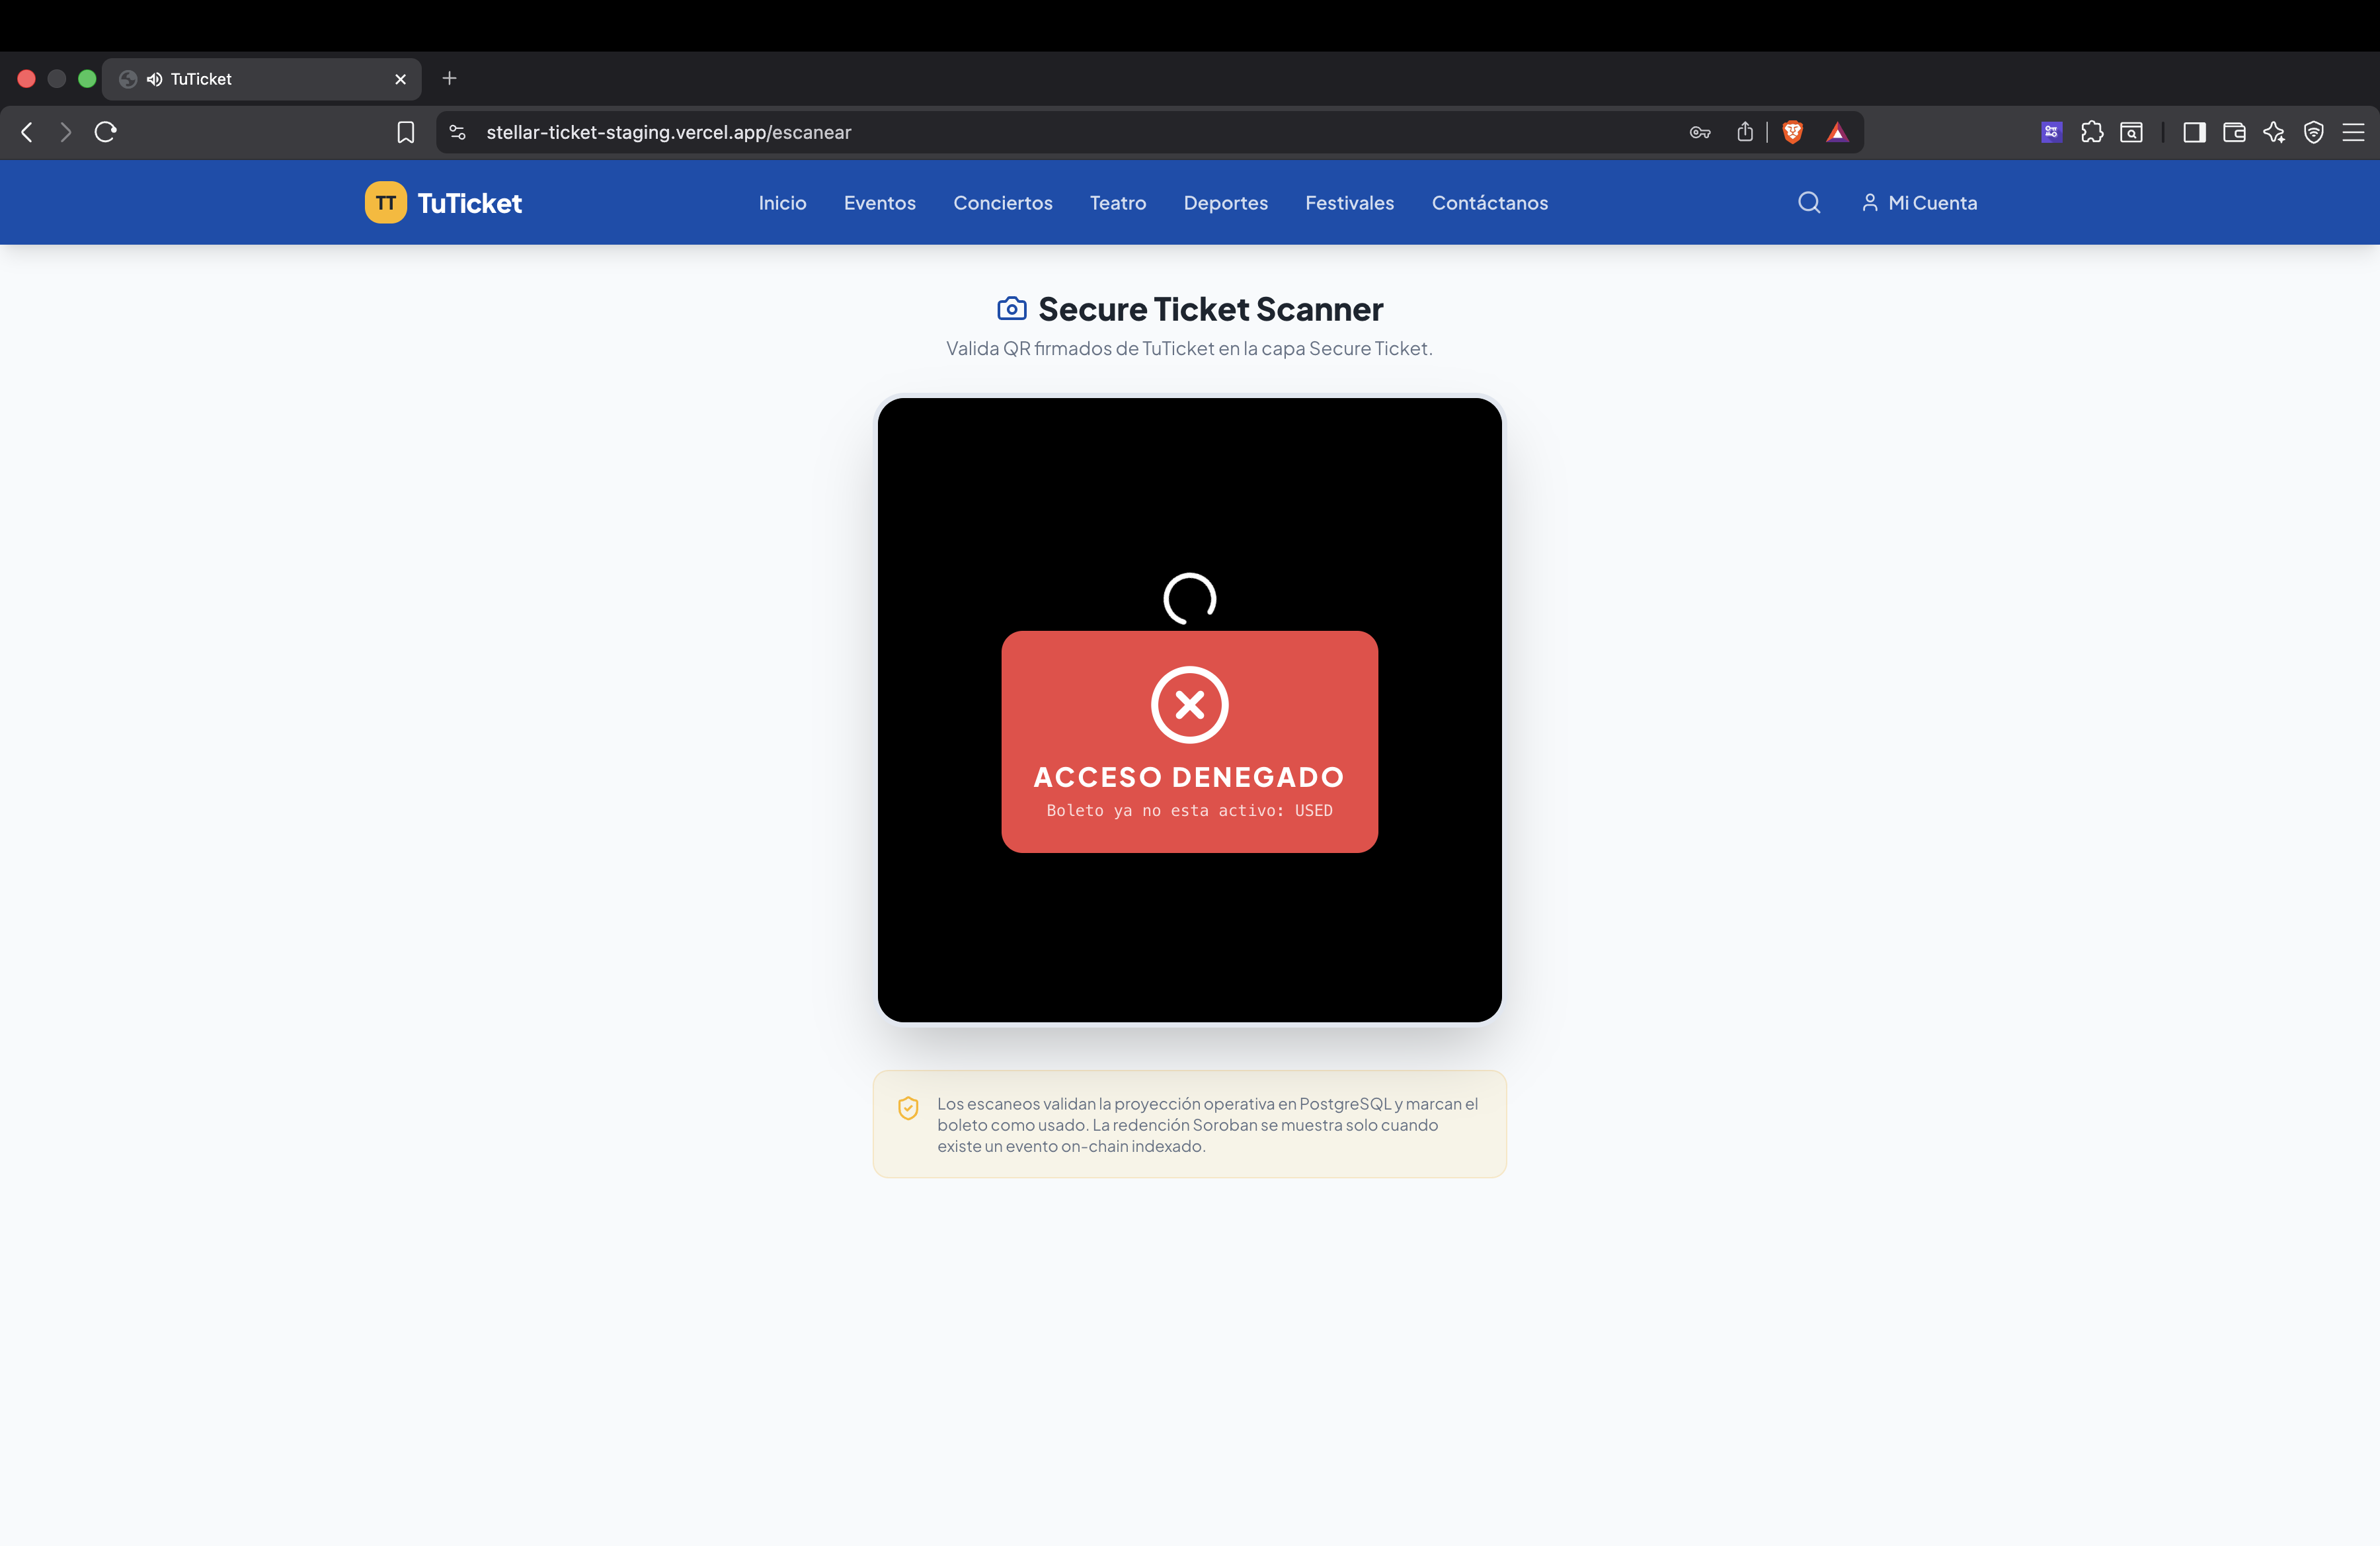
\includegraphics[width=0.92\textwidth]{Anexo/uat-08-rechazo-ticket-invalido.png}
\caption{Evidencia UAT-08: rechazo de ticket no válido}
\label{fig:evidencia-uat-08}
\end{figure}

\end{document}
